\documentclass[conference,final,11pt,technote,onecolumn]{IEEEtran}\usepackage[]{graphicx}\usepackage[]{color}
%% maxwidth is the original width if it is less than linewidth
%% otherwise use linewidth (to make sure the graphics do not exceed the margin)
\makeatletter
\def\maxwidth{ %
  \ifdim\Gin@nat@width>\linewidth
    \linewidth
  \else
    \Gin@nat@width
  \fi
}
\makeatother

\definecolor{fgcolor}{rgb}{0.345, 0.345, 0.345}
\newcommand{\hlnum}[1]{\textcolor[rgb]{0.686,0.059,0.569}{#1}}%
\newcommand{\hlstr}[1]{\textcolor[rgb]{0.192,0.494,0.8}{#1}}%
\newcommand{\hlcom}[1]{\textcolor[rgb]{0.678,0.584,0.686}{\textit{#1}}}%
\newcommand{\hlopt}[1]{\textcolor[rgb]{0,0,0}{#1}}%
\newcommand{\hlstd}[1]{\textcolor[rgb]{0.345,0.345,0.345}{#1}}%
\newcommand{\hlkwa}[1]{\textcolor[rgb]{0.161,0.373,0.58}{\textbf{#1}}}%
\newcommand{\hlkwb}[1]{\textcolor[rgb]{0.69,0.353,0.396}{#1}}%
\newcommand{\hlkwc}[1]{\textcolor[rgb]{0.333,0.667,0.333}{#1}}%
\newcommand{\hlkwd}[1]{\textcolor[rgb]{0.737,0.353,0.396}{\textbf{#1}}}%

\usepackage{framed}
\makeatletter
\newenvironment{kframe}{%
 \def\at@end@of@kframe{}%
 \ifinner\ifhmode%
  \def\at@end@of@kframe{\end{minipage}}%
  \begin{minipage}{\columnwidth}%
 \fi\fi%
 \def\FrameCommand##1{\hskip\@totalleftmargin \hskip-\fboxsep
 \colorbox{shadecolor}{##1}\hskip-\fboxsep
     % There is no \\@totalrightmargin, so:
     \hskip-\linewidth \hskip-\@totalleftmargin \hskip\columnwidth}%
 \MakeFramed {\advance\hsize-\width
   \@totalleftmargin\z@ \linewidth\hsize
   \@setminipage}}%
 {\par\unskip\endMakeFramed%
 \at@end@of@kframe}
\makeatother

\definecolor{shadecolor}{rgb}{.97, .97, .97}
\definecolor{messagecolor}{rgb}{0, 0, 0}
\definecolor{warningcolor}{rgb}{1, 0, 1}
\definecolor{errorcolor}{rgb}{1, 0, 0}
\newenvironment{knitrout}{}{} % an empty environment to be redefined in TeX

\usepackage{alltt}
% Possible options:
% draft, draftcls, draftclsnofoot, final
% 9pt, 10pt, 11pt, 12pt
% conference, journal, technote, peerreview, peerreviewca
% letterpaper, a4paper
% oneside, twoside  %%%% For printing/binding
% onecolumn, twocolumn
% %%%%%%%%%%%%%%%%%%%%%%%%%%%%%%%%%%%%%%%%%%%%%%%%%%%%%%%%%%%%%%%%%%%%%%%%

%% %%%%%%%%%%%%%%%%%% %%
%% Package inclusions %%
%% %%%%%%%%%%%%%%%%%% %%

\usepackage[backref]{hyperref}
%% For showing hyperlinks for citations + references, [option=backref] enables the backreferencing in the reference list.

\usepackage{cite}

% *** GRAPHICS RELATED PACKAGES ***
%\ifCLASSINFOpdf
  \usepackage{graphicx}
  % declare the path(s) where your graphic files are
   \graphicspath{{figures/}{images/}}
  % and their extensions so you won't have to specify these with
  % every instance of \includegraphics
  \DeclareGraphicsExtensions{.pdf,.jpg,.png,.jpeg}
%\else
  % or other class option (dvipsone, dvipdf, if not using dvips). graphicx
  % will default to the driver specified in the system graphics.cfg if no
  % driver is specified.
%  \usepackage[dvips]{graphicx}
  % declare the path(s) where your graphic files are
%  \graphicspath{{figures/}{images/}}
  % and their extensions so you won't have to specify these with
  % every instance of \includegraphics
%  \DeclareGraphicsExtensions{.eps,.pdf}
%\fi


% *** MATH PACKAGES ***
\usepackage[cmex10]{amsmath}


% *** SPECIALIZED LIST PACKAGES ***
\usepackage{algorithmic}

% *** ALIGNMENT PACKAGES ***
\usepackage{array}
\usepackage{mdwmath}
\usepackage{mdwtab}

\usepackage{eqparbox}

% *** SUBFIGURE PACKAGES ***
\usepackage[caption=false,font=footnotesize]{subfig}

% *** FLOAT PACKAGES ***
\usepackage{fixltx2e}

\usepackage{stfloats}

% *** PDF, URL AND HYPERLINK PACKAGES ***
\usepackage{url}
\usepackage{listings}
\usepackage{color}
\definecolor{dkgreen}{rgb}{0,0.6,0}
\definecolor{gray}{rgb}{0.5,0.5,0.5}
\definecolor{mauve}{rgb}{0.58,0,0.82}
\usepackage{tabularx}
\usepackage{amssymb}
\usepackage{cancel}


\usepackage{mathtools}
% correct bad hyphenation here
\hyphenation{op-tical net-works semi-conduc-tor}


\renewcommand{\thesection}{\arabic{section}}
\renewcommand{\thesubsection}{\thesection.\arabic{subsection}}
\renewcommand{\thesubsubsection}{\thesubsection.\thesection.\arabic{subsubsection}}

\renewcommand\thesectiondis{\arabic{section}}
\renewcommand\thesubsectiondis{\thesectiondis.\arabic{subsection}}
\renewcommand\thesubsubsectiondis{\thesubsectiondis.\arabic{subsubsection}}
\IfFileExists{upquote.sty}{\usepackage{upquote}}{}
\begin{document}


	
	\title{ \LARGE{Machine Learning Primer \emph{using R}}}
	\author{
  		\IEEEauthorblockN{Ashis Kumer Biswas\\\today}
  		\IEEEauthorblockA{}
		%   \and %Second authorblock
	}
	\date{\today}
	\maketitle


	\section{Vector Space}
	\label{term:vector_space}
Vector space, $V$ over a field $\mathbb{F}$ (e.g., $\mathbb{R}$) is a collection of vectors ($\vec v\in V$) allowing the two operations: vector addition and scalar multiplication satisfying the following properties:
\begin{itemize}
\item Commutativity: $\vec a + \vec b = \vec b + \vec a, \forall \vec a, \vec b\in V$
\item Associativity: $\vec a + (\vec b + \vec c) = (\vec a + \vec b) + \vec c, (k_1k_2)\vec a = k_1(k_2\vec b), \forall \vec a, \vec b, \vec c \in V, k_1,k_2\in \mathbb{F}$
\item Additive Identity: There exists an element $\vec 0\in V$ such that $\vec 0 + \vec a = \vec a, \forall \vec a\in V$
\item Additive Inverse: For every $\vec a\in V$, there exists $\vec b\in V$ such that $\vec a + \vec b = \vec 0$.
\item Multiplicative Identity: $1\vec a = \vec a, \forall \vec a\in V$
\item Distributivity: $k_1(\vec a + \vec b) = k_1\vec a + k_1\vec b$, and $(k_1 + k_2)\vec a = k_1\vec a + k_2\vec a$, $ \forall \vec a, \vec b\in V$, and $k_1, k_2\in \mathbb{F}$
\end{itemize}

Vector space possesses other properties too:
\begin{itemize}
\item Every vector $\vec a\in V$ has a unique additive identity.
\item Every vector $\vec a\in V$ has a unique additive inverse.
\item $0\vec a = \vec 0, \forall \vec a \in V$
\item $k_1\vec 0 = \vec 0, \forall k_1\in \mathbb{F}$.
\item $(-1)\vec a = -\vec a, \forall \vec a \in V$.
\end{itemize}

	\section{Vector Subspace}
	\label{term_vector_subspace}
Let $V$ be a \hyperref[term:vector_space]{vector space}	over $\mathbb{F}$, and let $U\subset V$ be a subset of $V$. Then $U$ is a said to be a subspace of $V$ if $U$ is a vector space over $\mathbb{F}$ under the same operations that make $V$ into a \hyperref[term:vector_space]{vector space} over $\mathbb{F}$. However, it will be enough to check whether the following three conditions hold.
\begin{itemize}
\item Additive identity: $\vec 0 \in U$
\item Closure under addition: $\vec a, \vec b \in U$ implies $\vec a + \vec b \in U$
\item Closure under scalar multiplication: $k_1 \in \mathbb{F}, \vec a\in U$ implies that $k_1\vec a \in U$.
\end{itemize}
	
	\section{Linear Span}
	\label{term:linear_span}
Let $V$ denote a \hyperref[term:vector_space]{vector space} over $\mathbb{F}$. Given vectors $\vec a_1, \vec a_2, \cdots, \vec a_m \in V$, and a vector $\vec a\in V$ is a linear combination of $(\vec a_1, \vec a_2, \cdots, \vec a_m)$ if there exist scalars $k_1, k_2, \cdots, k_m\in \mathbb{F}$ such that $\vec a = k_1\vec a_1 + k_2\vec a_2+ \cdots + k_m\vec a_m$. 

Thus, a linear span of a set of vectors $(\vec a_1, \vec a_2, \cdots, \vec a_m)$ is defined as:
\[ 
\text{span}(\vec a_1, \vec a_2, \cdots, \vec a_m) = \{ k_1\vec a_1 + k_2\vec a_2 + \cdots + k_m\vec a_m | k_1, k_2, \cdots, k_m\in \mathbb{F}\}
\]

If $V$ is a vector space, and $\vec a_1, \vec a_2, \cdots, \vec a_m\in V$, then 
\begin{itemize}
\item $\vec a_i \in \text{span}(\vec a_1, \vec a_2, \cdots, \vec a_m)$
\item $\text{span}(\vec a_1, \vec a_2, \cdots, \vec a_m)$ is a subspace of $V$.
\item If $U\subset V$ is a subspace such that $\vec a_1, \vec a_2, \cdots, \vec a_m\in U$, then $\text{span}(\vec a_1, \vec a_2, \cdots, \vec a_m)\subset U$
\end{itemize}
	
	

	\section{Linearly Independent Vectors}
	\label{term:linearly_independent_vectors}
Two rows, or two columns (a.k.a. vectors) of a matrix are called linearly dependent to each other if one is a multiple of the other. Three rows, or three columns of a matrix together are linearly dependent if one is linear combination of the other two. And so on... If you can not find this dependence among a set of rows or columns (a.k.a. vectors), then they are called linearly independent vectors.

\[
\vec a = \begin{pmatrix}
1\\
2\\
3
\end{pmatrix}, \vec b = \begin{pmatrix}
3\\
4\\
5
\end{pmatrix}, \vec c = \begin{pmatrix}
-5\\
2\\
0
\end{pmatrix}, \vec d = \begin{pmatrix}
10\\
-4\\
0
\end{pmatrix}, \vec e = \begin{pmatrix}
9\\
-6\\
-3
\end{pmatrix}
\]
Here, $\vec a$ and $\vec b$ are linearly dependent to each other, because $\vec b = \vec a + \vec 2$. $\vec c$ and $\vec d$ are linearly dependent to each other, because $\vec d = -2 . \vec c$. $\vec e$ is linearly dependent to $\vec a$ and $\vec d$, because $\vec e = \vec d - \vec a$. 

The following are the list of sets containing linearly independent vectors from the given five vectors:
\begin{itemize}
\item \{$\vec a, \vec c, \vec e$\}
\item \{$\vec a, \vec d$ \}
\item \{$\vec b, \vec c, \vec e$\}
\item \{$\vec b, \vec d, \vec e$\}
\item \{$\vec c, \vec e$\}
\item \{$\vec d, \vec e$\}
\end{itemize}

	\section{Basis}
	\label{term:basis}
A basis of a \hyperref[term:vector_space]{vector space} $V$ over a field $\mathbb{F}$ is a \hyperref[term:linearly_independent_vectors]{linearly independent} subset of $V$ that spans $V$. All bases for finite-dimensional vector spaces have the same length. This length will then be called the dimension of the \hyperref[term:vector_space]{vector space}.

A list of vectors $(\vec a_1, \vec a_2, \cdots, \vec a_m)$ is a basis for the finite-dimensional vector space $V$ if $(\vec a_1, \vec a_2, \cdots, \vec a_m)$ is linearly independent and $V = \text{span}(\vec a_1, \vec a_2, \cdots, \vec a_m)$

If $(\vec a_1, \vec a_2, \cdots, \vec a_m)$ forms a basis of $V$, then every vector $\vec a\in V$ can be uniquely written as a linear combination of $(\vec a_1, \vec a_2, \cdots, \vec a_m)$. That is, basis has the following two properties:

\begin{itemize}
\item Linear independence property: if $k_1\vec a_1 + k_2\vec a_2 + \cdots + k_m\vec a_m = 0$, then $k_1 = k_2 = \cdots = k_m = 0, \forall k_1, k_2, \cdots, k_m\in \mathbb{F}$
\item Spanning property: For every $\vec a\in V$ it is possible to choose $k_1, k_2, \cdots, k_m\in \mathbb{F}$ such that $\vec a = k_1\vec a_1 + k_2\vec a_2 + \cdots + k_m\vec a_m$.
\end{itemize}

Every finite-dimensional vector space has a basis.

Every linearly independent list of vectors in a finite-dimensional vector space $V$ can be extended to a basis of $V$.

Concisely, $B$ denotes a subset of a vector space $V$. Then $B$ is a basis iff any of the following equivalent conditions are met:
\begin{itemize}
\item $B$ is a minimal generating set of $V$, i.e., it is a generating set and no proper subset of $B$ is also a generating set.
\item $B$ is a maximal set of linearly independent vectors, i.e., it is a linearly independent set but no other linearly independent set contains it as a proper subset.
\item Every vector in $V$ can be expressed as a linear combination of vectors in $B$ in a unique way. 
\end{itemize}
\begin{figure}[!h]
\centering
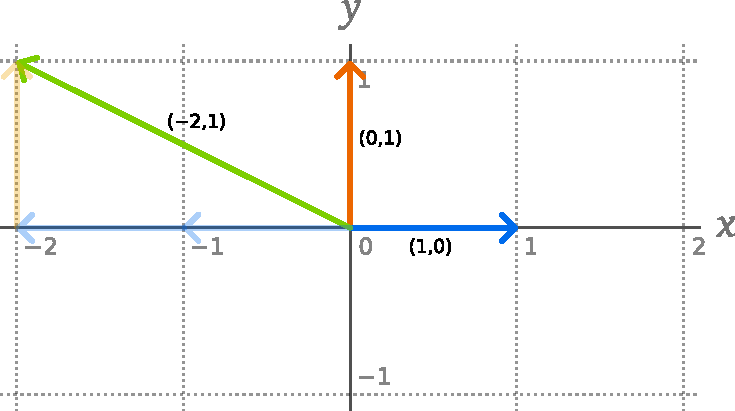
\includegraphics[scale=1]{basis_graph.pdf}
\caption{\label{fig:basis}This picture illustrates the standard basis in $\mathbb{R}^2$. The blue and orange vectors are the elements of the basis; the green vector can be given in terms of the basis vectors, and so is linearly dependent upon them. This picture illustrates how two vectors in $\mathbb{R}^2$ (or $\mathbb{R} \times \mathbb{R}$) can be written in terms of the standard basis. $B = \{(1,0), (0,1)\}$. Notice how $\text{span}(B) = \mathbb{R}^2$, and how (-2, 1) = (-2)(1,0) + (1)(0,1). Reference \url{https://en.wikipedia.org/wiki/Basis_(linear_algebra)} (Last accessed: 10/28/2014, 2:04AM)}
\end{figure}

Figure \ref{fig:basis} illustrates a geometric interpretation of the basis concept.
	
	\section{Rank of a Matrix}
	\label{term:rank_of_a_matrix}
The number of \hyperref[term:linearly_independent_vectors]{linearly independent} rows and/or columns is the rank of the matrix. If all of the rows, as well as all of the columns are \hyperref[term:rank_of_a_matrix]{linearly independent}, then the matrix is called full rank.

A set (i.e., family) of vectors is linearly dependent if a member vector is in the linear span of the rest of the family, i.e., a member vector can be represented by a linear combination of the rest of the family. 

A set of vectors which is linearly independent and spans some vector space, forms a \hyperref[term:basis]{basis} for that vector space. For example, the vector space of all polynomials in $x$ over the reals has the infinite subset $\{1, x, x^2, x^3, \cdots\}$ as a basis.

	\section{Singular Matrix}
	\label{term:singular_matrix}
The square matrix which is not \hyperref[term:rank_of_a_matrix]{full rank}, is called a singular matrix. That is, one or more rows and/or columns of the matrix are \hyperref[term:linearly_independent_vectors]{linearly dependent}. A singular matrix is not invertible. Only the non-singular matrices are invertible.

Singular matrices are also called the degenerate matrices.

A square matrix is singular iff the determinant is 0.

If a matrix $A$ is singular, so does the $A^T$. Similarly, if a matrix $A$ is non-singular, so does the matrix $A^T$.

Other properties of invertible (i.e., non-singular, or non-degenerate) matrices:
\begin{itemize}
\item $(A^{-1})^{-1} = A$
\item $(k_1A)^{-1} = \frac{1}{k_1}A^{-1}$ for any constant $k_1$
\item $(A^T)^{-1} = (A^{-1})^T$
\item For any invertible matrices $A$ and $B$, $(AB)^{-1} = B^{-1}A^{-1}$. Or, more generally, for the invertible matrices $A_1, A_2, \cdots, A_m$, $(A_1A_2\cdots A_m)^{-1} = A^{-1}_m\cdots A^{-1}_2A^{-1}_1$
\item $\text{det}(A^{-1}) = (\text{det}(A))^{-1}$
\end{itemize}
	\section{Idempotent Matrix}
	\label{term:idempotent_matrix}
	It is a matrix when multiplied to itself produces itself\cite{chiang2005fundamental}. The matrix $A$ is idempotent if $AA=A$. And obviously the matrix $A$ should be a square matrix. Except the \hyperref[term:identity_matrix]{identity matrix}, all the idempotent matrices are \hyperref[term:singular_matrix]{singular}. 
	
	\section{Diagonal Matrix}
	\label{term:diagonal_matrix}
It is a square matrix in which the entries outside the main diagonal (i.e, top-left to bottom-right) are all zero. The diagonal entries themselves may or may not be zero.

Properties of the diagonal matrices are:
\begin{itemize}
\item $\text{det}(\text{diag}(a_1, a_2\cdots, a_n)) = a_1a_2\cdots a_n$
\end{itemize}
	
	\section{Identity Matrix}
	\label{term:identity_matrix}
It is like 1 in scalar sense. You multiply anything to 1, you get exactly what you multiplied with it. So, for any given square matrix $A\in\mathbb{R}^{n\times n}$, multiplying it with the identity matrix of same dimension would produce the same matrix $A$.
\begin{equation}
IA = AI = A
\end{equation}
where,
\[ 
A =
 \begin{pmatrix}
  a_{1,1} & a_{1,2} & \cdots & a_{1,n} \\
  a_{2,1} & a_{2,2} & \cdots & a_{2,n} \\
  \vdots  & \vdots  & \ddots & \vdots  \\
  a_{n,1} & a_{n,2} & \cdots & a_{n,n}
 \end{pmatrix}_{n\times n}, \qquad I = I_n = 
 \begin{pmatrix}
 	1 & 0 & \cdots & 0 \\
 	0 & 1 & \cdots & 0 \\
 	\vdots & \vdots & 1 & \vdots \\
 	0 & 0 & \cdots & 1
 \end{pmatrix}_{n\times n}
\]
Here, the identity matrix is also known as the ``unit matrix''\cite{akivis2012introduction}.
Identity matrix can also be described using the diagonal matrix operator:
\[
diag(I_n) = \begin{pmatrix}
			1 & 1 & \cdots & 1
			\end{pmatrix}_{n}
\]

If multiplication of two square matrices $X$ and $Y$ yields the identity matrix $I$, then the two matrices $X$ and $Y$ would be called the inverse matrix to each other.
\begin{eqnarray}
\nonumber X Y = I \Rightarrow X = Y^{-1}, \text{ and } Y = X^{-1}
\end{eqnarray}

The identity matrix is its own inverse.

The identity matrix is an \hyperref[term:idempotent_matrix]{idempotent matrix}.

The identity matrix is the only \hyperref[term:idempotent_matrix]{idempotent matrix} having \hyperref[term:rank_of_a_matrix]{full-rank}. 

\begin{knitrout}
\definecolor{shadecolor}{rgb}{0.969, 0.969, 0.969}\color{fgcolor}\begin{kframe}
\begin{alltt}
\hlstd{A} \hlkwb{=} \hlkwd{matrix}\hlstd{(}\hlkwd{c}\hlstd{(}\hlnum{1}\hlstd{,}\hlnum{2}\hlstd{,}\hlnum{3}\hlstd{,}\hlnum{4}\hlstd{,}\hlnum{5}\hlstd{,}\hlnum{6}\hlstd{,}\hlnum{7}\hlstd{,}\hlnum{8}\hlstd{,}\hlnum{9}\hlstd{),}\hlkwc{nrow} \hlstd{=} \hlnum{3}\hlstd{,}\hlkwc{ncol} \hlstd{=} \hlnum{3}\hlstd{,}\hlkwc{byrow}\hlstd{=} \hlnum{TRUE}\hlstd{)}
\hlstd{A} \hlcom{#The matrix A}
\end{alltt}
\begin{verbatim}
##      [,1] [,2] [,3]
## [1,]    1    2    3
## [2,]    4    5    6
## [3,]    7    8    9
\end{verbatim}
\begin{alltt}
\hlstd{I} \hlkwb{=} \hlkwd{matrix}\hlstd{(}\hlkwd{c}\hlstd{(}\hlnum{1}\hlstd{,}\hlnum{0}\hlstd{,}\hlnum{0}\hlstd{,}\hlnum{0}\hlstd{,}\hlnum{1}\hlstd{,}\hlnum{0}\hlstd{,}\hlnum{0}\hlstd{,}\hlnum{0}\hlstd{,}\hlnum{1}\hlstd{),}\hlkwc{nrow} \hlstd{=} \hlnum{3}\hlstd{,}\hlkwc{ncol} \hlstd{=} \hlnum{3}\hlstd{,} \hlkwc{byrow} \hlstd{=}\hlnum{TRUE}\hlstd{)}
\hlstd{I}
\end{alltt}
\begin{verbatim}
##      [,1] [,2] [,3]
## [1,]    1    0    0
## [2,]    0    1    0
## [3,]    0    0    1
\end{verbatim}
\begin{alltt}
\hlcom{#You could also use the matlab command eye}
\hlkwd{library}\hlstd{(matlab)}
\hlstd{I} \hlkwb{=} \hlkwd{eye}\hlstd{(}\hlnum{3}\hlstd{)} \hlcom{#dimension 3x3}
\hlcom{#Now do the multiplication}
\hlstd{A} \hlopt \hlstd{I}
\end{alltt}
\begin{verbatim}
##      [,1] [,2] [,3]
## [1,]    1    2    3
## [2,]    4    5    6
## [3,]    7    8    9
\end{verbatim}
\begin{alltt}
\hlcom{#Multiply again}
\hlstd{I} \hlopt \hlstd{A}
\end{alltt}
\begin{verbatim}
##      [,1] [,2] [,3]
## [1,]    1    2    3
## [2,]    4    5    6
## [3,]    7    8    9
\end{verbatim}
\begin{alltt}
\hlcom{#Define X matrix}
\hlstd{X} \hlkwb{=} \hlkwd{matrix}\hlstd{(}\hlkwd{c}\hlstd{(}\hlnum{1}\hlstd{,}\hlnum{3}\hlstd{,}\hlnum{2}\hlstd{,}\hlopt{-}\hlnum{1}\hlstd{,}\hlnum{5}\hlstd{,}\hlnum{0}\hlstd{,}\hlnum{7}\hlstd{,}\hlnum{7}\hlstd{,}\hlnum{1}\hlstd{),}\hlkwc{nrow} \hlstd{=} \hlnum{3}\hlstd{,}\hlkwc{ncol} \hlstd{=} \hlnum{3}\hlstd{,}\hlkwc{byrow}\hlstd{=} \hlnum{TRUE}\hlstd{)}
\hlstd{X} \hlcom{#The X matrix}
\end{alltt}
\begin{verbatim}
##      [,1] [,2] [,3]
## [1,]    1    3    2
## [2,]   -1    5    0
## [3,]    7    7    1
\end{verbatim}
\begin{alltt}
\hlcom{#Calculate the inverse of X}
\hlstd{Y} \hlkwb{=} \hlkwd{solve}\hlstd{(X)}
\hlcom{#Now, let's multiply X and Y}
\hlstd{X} \hlopt \hlstd{Y} \hlcom{#It's identity (or very very close to the identity matrix, isn't it?)}
\end{alltt}
\begin{verbatim}
##              [,1]          [,2] [,3]
## [1,] 1.000000e+00  5.551115e-17    0
## [2,] 1.387779e-17  1.000000e+00    0
## [3,] 0.000000e+00 -8.326673e-17    1
\end{verbatim}
\begin{alltt}
\hlcom{#Let's get the rank of a matrix}
\hlkwd{library}\hlstd{(Matrix)}
\hlkwd{rankMatrix}\hlstd{(A)[}\hlnum{1}\hlstd{]} \hlcom{#rank of matrix A, should be == 2}
\end{alltt}
\begin{verbatim}
## [1] 2
\end{verbatim}
\begin{alltt}
\hlkwd{rankMatrix}\hlstd{(I)[}\hlnum{1}\hlstd{]} \hlcom{#rank of matrix I, should be == 3}
\end{alltt}
\begin{verbatim}
## [1] 3
\end{verbatim}
\begin{alltt}
\hlkwd{rankMatrix}\hlstd{(X)[}\hlnum{1}\hlstd{]} \hlcom{#rank of matrix X, should be == 3}
\end{alltt}
\begin{verbatim}
## [1] 3
\end{verbatim}
\begin{alltt}
\hlkwd{rankMatrix}\hlstd{(Y)[}\hlnum{1}\hlstd{]} \hlcom{#rank of matrix Y, should be == 3}
\end{alltt}
\begin{verbatim}
## [1] 3
\end{verbatim}
\begin{alltt}
\hlcom{#Done.}
\end{alltt}
\end{kframe}
\end{knitrout}

\section{Triangular Matrix}
\label{term:triangular_matrix}
A square matrix is called lower triangular matrix if all the entries above the main diagonal (i.e., from top-left to bottom-right) are zero\cite{wiki:TriangularMatrix}. For instance,
\[
L = \begin{pmatrix}
    	l_{1,1} &         &         &           &   0    \\
      l_{2,1} & l_{2,2} &         &           &        \\
      l_{3,1} & l_{3,2} & \ddots  &           &        \\
      \vdots  & \vdots  & \ddots  & \ddots    &        \\
      l_{n,1} & l_{n,2} & \cdots  & l_{n,n-1} & l_{n,n}
			\end{pmatrix} 
\]

A square matrix is called upper triangular if all the entries below the main diagonal are zero. For example,
\[
U = \begin{pmatrix}
      u_{1,1} & u_{1,2} & u_{1,3} & \cdots    &   u_{1,n}    \\
              & u_{2,2} & u_{2,3} & \cdots    &   u_{2,n}    \\
              &         & \ddots  & \ddots    &   \vdots     \\
              &         &         & \ddots    &   u_{n-1,n}  \\
      0       &         &         &           &   u_{n,n}
			\end{pmatrix} 
\]

A triangular matrix is one that is either lower triangular or upper traingular.

A matrix that is both upper and lower triangular matrix is called a \hyperref[term:diagonal_matrix]{diagonal matrix}.

Determinant of a triangular matrix ($L$ or $U$) is the product of all the elements in the main diagonal. That is, 
\begin{eqnarray}
\nonumber \text{det}(L) = l_{1,1}\times l_{2,2}\times l_{3,3}\times \cdots \times l_{n,n} = \prod_{i=1}^nl_{i,i}\\
\nonumber \text{det}(U) = u_{1,1}\times u_{2,2}\times u_{3,3}\times \cdots \times u_{n,n} = \prod_{i=1}^nu_{i,i}
\end{eqnarray}

\section{Row Echelon Form}
\label{term:row_echelon_form}
If you apply \hyperref[term:gauss_jordan_elimination_algorithm]{Gaussian elimination} on a matrix, the resulting  matrix will be in row echelon form. A matrix is in row echelon form if
\begin{itemize}
  \item All nonzero rows (i.e.,rows with at least one nonzero element) are above any rows of all zeros (all zero rows, if any, belong at the bottom of the matrix)
  \item The leading coefficient (i.e., the first nonzero number from the left, also called the pivot) of nonzero row is always strictly to the right of the leading coefficient of the row above it.
  \item All entries in a column below a leading entry are zeros (implied by the first two criteria).
\end{itemize}
This is an example of $3\times 6$ matrix in row echelon form:
\[ 
\begin{pmatrix}
    	3 & -9 & 12 & -9 & 6 & 15 \\
      0 & 1  & -2 & 2 & 1  & -3\\
      0 & 0 & 0 & 0 & 1 & 4
			\end{pmatrix}
\]

A matrix is in reduced row echelon form (a.k.a., row canonical form) if it satisfied the following conditions:
\begin{itemize}
  \item It is in row echelon form
  \item Every pivot (i.e., leading coefficient of the row) is 1, and is the only nonzero entry in its column.
\end{itemize}
You can create the reduced row echelon form of a matrix from its echelon form: beginning with the rightmost leading entry, and working upwards to the left, create zeros above each leading entry and scale rows to transform each leading entry into 1.

Let's work with the $3\times 6$ matrix above:
\begin{eqnarray}
\nonumber \begin{pmatrix}
      3 & -9 & 12 & -9 & 6 & 15 \\
      0 & 1  & -2 & 2 & 1  & -3\\
      0 & 0 & 0 & 0 & 1 & 4
			\end{pmatrix} \xRightarrow{9R_2+R_1\rightarrow R_1} \begin{pmatrix}
      3 & 0 & -6 & 9 & 0 & -72 \\
      0 & 1  & -2 & 2 & 1  & -3\\
      0 & 0 & 0 & 0 & 1 & 4
  		\end{pmatrix}\\
\nonumber \begin{pmatrix}
      3 & 0 & -6 & 9 & 0 & -72 \\
      0 & 1  & -2 & 2 & 1  & -3\\
      0 & 0 & 0 & 0 & 1 & 4
    	\end{pmatrix} \xRightarrow{\frac{1}{3}R_1\rightarrow R_1} \begin{pmatrix}
      1 & 0 & -2 & 3 & 0 & -24 \\
      0 & 1  & -2 & 2 & 1  & -3\\
      0 & 0 & 0 & 0 & 1 & 4
    	\end{pmatrix}
\end{eqnarray}
\section{Gauss-Jordan Elimination Algorithm}
\label{term:gauss_jordan_elimination_algorithm}
This method is a sequence of operations performed on the coefficient matrix corresponding to a system of linear equations to solve it\cite{wiki:GaussianElimination}. However, the method is also useful --
\begin{itemize}
  \item To find rank of a matrix
  \item To calculate the determinant of a matrix
  \item To calculate the inverse of an invertible square matrix.
\end{itemize}

To perform row reduction on a matrix, one uses a sequence of elementary row operations to modify the matrix until the lower left-hand corner of the matrix is filled with zeros. There are three types of elementary row operations:
\begin{enumerate}
  \item \textbf{Row Switching}: A row within the matrix can be switched to another row. $R_i \leftrightarrow R_j$.
  \item \textbf{Row Multiplication}: Each element in a row can be multiplied by a non-zero constant. That is, $kR_i \rightarrow R_i$, where $k\neq 0$.
  \item \textbf{Row Addition}: A row can be replaced by the sum of that row and a multiple of another row. That is, $R_i + kR_j \rightarrow R_i$, where $i\neq j$
\end{enumerate}

Using these operations, a matrix can always be transformed into an \hyperref[term:triangular_matrix]{upper triangular matrix}, and in fact one that is in \hyperref[term:row_echelon_form]{row echelon form}. The steps required upto this is called Gaussian Elimination. However, the steps of row reduction until the matrix becomes the \hyperref[term:row_echelon_form]{reduced row echelon form} is called Gauss-Jordan Elimination, to distinguish it from stopping after reaching the echelon form.

\subsection{Solving system of linear equations}
\label{term:gauss_jordan_elimination_algorithm_solve_systems}
Given the following system of linear equations:
\begin{eqnarray}
2x + y - z &=& 8\qquad (L_1)\\
-3x -y + 2z &=& -11 \qquad (L_2)\\
-2x + y + 2z &=& -3 \qquad (L_3)
\end{eqnarray}

The table below is the row reduction process applied to the associated augmented matrix.
\begin{eqnarray}
\nonumber \left[ \begin{array}{ccc|c}
2 & 1 & -1 & 8\\
-3 & -1 & 2 & -11\\
-2 & 1 & 2 & -3
\end{array} \right] \xRightarrow{\substack{L_2+\frac{3}{2}L_1 \rightarrow L_2\\ L_3+L_1\rightarrow L_3}} \left[ \begin{array}{ccc|c}
2 & 1 & -1 & 8\\
0 & \frac{1}{2} & \frac{1}{2} & 1\\
0 & 2 & 1 & 5
\end{array} \right]\\
\nonumber \left[ \begin{array}{ccc|c}
2 & 1 & -1 & 8\\
0 & \frac{1}{2} & \frac{1}{2} & 1\\
0 & 2 & 1 & 5
\end{array} \right] \xRightarrow{L_3+(-4)L_2 \rightarrow L_3} \left[ \begin{array}{ccc|c}
2 & 1 & -1 & 8\\
0 & \frac{1}{2} & \frac{1}{2} & 1\\
0 & 0 & -1 & 1
\end{array} \right]\\
\nonumber \left[ \begin{array}{ccc|c}
2 & 1 & -1 & 8\\
0 & \frac{1}{2} & \frac{1}{2} & 1\\
0 & 0 & -1 & 1
\end{array} \right] \xRightarrow{\substack{L_2+\frac{1}{2}L_3\rightarrow L_2\\ L_1-L_3\rightarrow L_1}}  \left[ \begin{array}{ccc|c}
2 & 1 & 0 & 7\\
0 & \frac{1}{2} & 0 & \frac{1}{2}\\
0 & 0 & -1 & 1
\end{array} \right]\\
\nonumber \left[ \begin{array}{ccc|c}
2 & 1 & 0 & 7\\
0 & \frac{1}{2} & 0 & \frac{1}{2}\\
0 & 0 & -1 & 1
\end{array} \right] \xRightarrow{\substack{2L_2 \rightarrow L_2\\ -L_3\rightarrow L_3}} \left[ \begin{array}{ccc|c}
2 & 1 & 0 & 7\\
0 & 1 & 0 & 3\\
0 & 0 & 1 & -1
\end{array} \right] \\
\nonumber \left[ \begin{array}{ccc|c}
2 & 1 & 0 & 7\\
0 & 1 & 0 & 3\\
0 & 0 & 1 & -1
\end{array} \right] \xRightarrow{\substack{L_1-L_2\rightarrow L_1\\ \frac{1}{2}L_1\rightarrow L_1}}\left[ \begin{array}{ccc|c}
1 & 0 & 0 & 2\\
0 & 1 & 0 & 3\\
0 & 0 & 1 & -1
\end{array} \right]
\end{eqnarray}
So, the solution to the given system is:
\begin{eqnarray}
\nonumber \left[  \begin{array}{c} 
x\\
y\\
z
\end{array} \right] = \left[ 
\begin{array}{c}
2\\
3\\
-1
\end{array}
\right]
\end{eqnarray}

\subsection{Computing Determinant of matrix}
\label{term:gauss_jordan_elimination_algorithm_compute_determinant}
Let's look at how the elementary row operations on a square matrix $A\in \mathbb{R}^{n\times n}$ affect the determinant of that matrix:
\begin{itemize}
	\item \textbf{Row switching}: Everytime you switch any two rows $R_i$ and $R_j$ of matrix $A$, you will have the same determinant with opposite sign, i.e., $\text{det}(A)\xrightarrow{\substack{R_i \rightarrow R_j\\ R_j \rightarrow R_i}} (-1)\times \text{det}(A)$.
	\item \textbf{Row multiplication}: Multiplying a row by a nonzero scalar $k$ multiplies the determinant by the same scalar. That is, $\text{det}(A) \xrightarrow{k R_i} k \text{det}(A)$
	\item \textbf{Row addition}: Adding to one row a scalar multiple of another does not change the determinant. That is, $\text{det}(A) \xrightarrow{R_i+k R_j\rightarrow R_i} \text{det}(A)$ 
\end{itemize}
Now let's do two examples.

Example 1: Compute the determinant of 
\[ A =  \left[ \begin{array}{ccc}
3 & -17 & 4\\
0 & 5 & 1\\
0 & 0 & -2
\end{array} \right] \]
Ans: Since the matrix is upper triangular, the determinant is very easy to calculate, which is the product of all the elements of its main diagonal. So, $\text{det}(A) = 3\times 5 \times (-2) = -30$

Example 2: Compute the determinant of 
\[ 
	B = \left[ 
		\begin{array}{ccc}
			1 & -3 & 0\\
			-2 & 4 & 1\\
			5 & -2 & 2
		\end{array}
	\right]
\]
Ans: Let's apply Gaussian Elimination to find the determinant.
 \begin{eqnarray}
 \nonumber \text{det}\left( \left[ 
 		\begin{array}{ccc}
 			1 & -3 & 0\\
 			-2 & 4 & 1\\
 			5 & -2 & 2
 		\end{array}
 	\right]\right) \stackrel{\substack{R_2+2R_1\rightarrow R_2\\R_3-5R_1\rightarrow R_3}}{=\joinrel=\joinrel=\joinrel=\joinrel=\joinrel=\joinrel=\joinrel=} \text{det}\left( \left[ 
 		\begin{array}{ccc}
 			1 & -3 & 0\\
 			0 & -2 & 1\\
 			0 & 13 & 2
 		\end{array}
 	\right]\right)\\
\nonumber \text{det}\left( \left[ 
 		\begin{array}{ccc}
 			1 & -3 & 0\\
 			0 & -2 & 1\\
 			0 & 13 & 2
 		\end{array}
 	\right]\right) \stackrel{\substack{R_3+\frac{13}{2}R_2\rightarrow R_3}}{=\joinrel=\joinrel=\joinrel=\joinrel=\joinrel=\joinrel=\joinrel=} 
 	\text{det}\left( \left[ 
 		\begin{array}{ccc}
 			1 & -3 & 0\\
 			0 & -2 & 1\\
 			0 & 0 & \frac{17}{2}
 		\end{array}
 		\right] \right)
\end{eqnarray}

Since, the echelon form is an upper triangular matrix, then the determinant is given by $1\times (-2)\times \frac{17}{2} = -17$.


\subsection{Computing rank of matrix}
\label{term:gauss_jordan_elimination_algorithm_compute_rank}
The Gaussian elimination algorithm can be applied to any $m\times n$ matrix $A$. In this way, for example, some $6\times 9$ matrices can be transformed to a matrix that has a row echelon form like:
\[ 
T = \begin{pmatrix}
a & * & * & * & * & * & * & * & *\\
0 & 0 & b & * & * & * & * & * & *\\
0 & 0 & 0 & c & * & * & * & * & *\\
0 & 0 & 0 & 0 & 0 & 0 & d & * & *\\
0 & 0 & 0 & 0 & 0 & 0 & 0 & 0 & e\\
0 & 0 & 0 & 0 & 0 & 0 & 0 & 0 & 0
\end{pmatrix}
\]
where the $*$'s are arbitrary entries and $a,b,c,d,e$ are non-zero entries. This echelon matrix $T$ contains a wealth of information about $A$, which are--
\begin{itemize}
	\item $\text{rank}(A) = 5$, since there are 5 non-zero rows in $T$.
	\item The vector space spanned by the columns of $A$ has a basis consisting of the first, third, fourth, seventh and ninth columns of $A$ (i.e., the columns of $a,b,c,d,e$ in $T$), and the $*$'s tell you how the other columns of $A$ can be written as linear combinations of the basis columns.
\end{itemize}
Now, let's do an example:
Example: compute rank of the following matrix $B$:
\[ 
B = \begin{pmatrix}
2 & 1 & 3 & 2\\
3 & 2 & 5 & 1\\
-1 & 1 & 0 & -7\\
3 & -2 & 1 & 17\\
0 & 1 & 1 & -4
\end{pmatrix}
\]
Ans: We'll apply Gaussian Elimination to find out the rank of the $B$ matrix.
\begin{eqnarray}
\nonumber \begin{pmatrix}
2 & 1 & 3 & 2\\
3 & 2 & 5 & 1\\
-1 & 1 & 0 & -7\\
3 & -2 & 1 & 17\\
0 & 1 & 1 & -4
\end{pmatrix} \xRightarrow{\substack{R_2+3R_3\rightarrow R_2\\R_3+\frac{1}{2}R_1\rightarrow R_3\\ R_4+3R_3\rightarrow R_4}} \begin{pmatrix}
2 & 1 & 3 & 2\\
0 & 5 & 5 & -20\\
0 & \frac{3}{2} & \frac{3}{2} & -6\\
0 & 1 & 1 & -10\\
0 & 1 & 1 & -4
\end{pmatrix}\\
\nonumber \begin{pmatrix}
2 & 1 & 3 & 2\\
0 & 5 & 5 & -20\\
0 & \frac{3}{2} & \frac{3}{2} & -6\\
0 & 1 & 1 & -10\\
0 & 1 & 1 & -4
\end{pmatrix} \xRightarrow{\substack{R_3+\left(\frac{-3}{2}\right)R_4\rightarrow R_3\\R_4+(-1)R_5\rightarrow R_4\\R_5+(-1)R_4\rightarrow R_5}}  \begin{pmatrix}
2 & 1 & 3 & 2\\
0 & 5 & 5 & -20\\
0 & 0 & 0 & 15\\
0 & 0 & 0 & -6\\
0 & 0 & 0 & 6
\end{pmatrix}\\
\nonumber \begin{pmatrix}
2 & 1 & 3 & 2\\
0 & 5 & 5 & -20\\
0 & 0 & 0 & 15\\
0 & 0 & 0 & -6\\
0 & 0 & 0 & 6
\end{pmatrix} \xRightarrow{\substack{R_3+\frac{15}{6}R_4\rightarrow R_3\\R_4+R_5\rightarrow R_4\\R_5+R_4\rightarrow R_5}} \begin{pmatrix}
\mathbf{2} & 1 & 3 & 2\\
0 & \mathbf{5} & 5 & -20\\
0 & 0 & 0 & 0\\
0 & 0 & 0 & 0\\
0 & 0 & 0 & 0
\end{pmatrix}
\end{eqnarray}
We see that there are only two pivots in the echelon matrix, so the $\text{rank}(B) = 2$. And hence, the first and second columns (i.e., the columns containing the two pivots) form the basis. The two basis vectors (first \& second columns of $B$ in this example) spans all the vectors represented in the matrix $B$. We can represent all the other columns of $B$ by linear combination of the two basis vectors, $\vec v_1=\begin{pmatrix}2\\3\\-1\\3\\0\end{pmatrix}, \vec v_2=\begin{pmatrix}1\\2\\1\\-2\\1\end{pmatrix}$. Let's try it:
\begin{itemize}
	\item The third column of $B$ = $\begin{pmatrix}3\\5\\0\\1\\1\end{pmatrix} = \vec v_1 + \vec v_2 = \begin{pmatrix}2\\3\\-1\\3\\0\end{pmatrix} + \begin{pmatrix}1\\2\\1\\-2\\1\end{pmatrix}$
	\item The fourth column of $B$ = $\begin{pmatrix}2\\1\\-7\\17\\-4\end{pmatrix} = 3\vec v_1 -4\vec v_2 = 3 \begin{pmatrix}2\\3\\-1\\3\\0\end{pmatrix} - 4 \begin{pmatrix}1\\2\\1\\-2\\1\end{pmatrix} = \begin{pmatrix}6\\9\\-3\\9\\0\end{pmatrix} + \begin{pmatrix}-4\\-8\\-4\\8\\-4\end{pmatrix}$
\end{itemize}

\subsection{Computing inverse of matrix}
\label{term:term:gauss_jordan_elimination_algorithm_compute_inverse}
The variant of the Gaussian elimination, called the Gauss-Jordan elimination algorithm can be used to find the inverse of a matrix, $A\in \mathbb{R}^{n\times n}$, if the matrix is invertible. 

First, the $n\times n$ identity matrix $I$ is augmented to the right of $A$, forming a block matrix $[A | I] \in \mathbb{R}^{n\times 2n}$.

Then by applying elementary row operations on the block matrix, we find the ``reduced row echelon form''.

The matrix $A$ is invertible if and only if the left block can be reduced to the identiy matrix $I$; in this case the right block of the final matrix is the result inverse matrix of $A$, which is $A^{-1}$. If the algorithm can not reduce the left block to $I$, then $A$ must not be invertible.

Let's work with an example. Consider the matrix $A$:
\begin{eqnarray}
\nonumber A = \begin{pmatrix}
2 & -1 & 0\\
-1 & 2 & -1\\
0 & -1 & 2
\end{pmatrix}
\end{eqnarray}
We need to find out $A^{-1}$ using the Gauss-Jordan Elimination Algorithm. Let's first build the augmented block matrix, and perform the elementary row operations on it:

 \begin{eqnarray}
 \nonumber [A | I] = \left[ \begin{array}{ccc|ccc}
 2 & -1 & 0 & 1 & 0 & 0\\
 -1 & 2 & -1 & 0 & 1 & 0\\
 0 & -1 & 2 & 0 & 0 & 1
 \end{array} \right] \xRightarrow{\frac{1}{2}R_1+R_2\rightarrow R_2}\left[ \begin{array}{ccc|ccc}
 2 & -1          & 0  &    1        & 0 & 0\\
 0 & \frac{3}{2} & -1 & \frac{1}{2} & 1 & 0\\
 0 & -1 & 2 & 0 & 0 & 1
 \end{array}\right]\\
 \nonumber \left[ \begin{array}{ccc|ccc}
 2 & -1          & 0  &    1        & 0 & 0\\
 0 & \frac{3}{2} & -1 & \frac{1}{2} & 1 & 0\\
 0 & -1 & 2 & 0 & 0 & 1
 \end{array}\right] \xRightarrow{\frac{3}{2}R_3+R_2\rightarrow R_3} \left[ \begin{array}{ccc|ccc}
 2 & -1          & 0  &    1        & 0 & 0\\
 0 & \frac{3}{2} & -1 & \frac{1}{2} & 1 & 0\\
 0 & 0 & 2 & \frac{1}{2} & 1 & \frac{3}{2}
 \end{array}\right] \\
 \nonumber \left[ \begin{array}{ccc|ccc}
 2 & -1          & 0  &    1        & 0 & 0\\
 0 & \frac{3}{2} & -1 & \frac{1}{2} & 1 & 0\\
 0 & 0 & 2 & \frac{1}{2} & 1 & \frac{3}{2}
 \end{array}\right] \xRightarrow{\substack{\frac{1}{2}R_3+R_2\rightarrow R_2}} \left[ \begin{array}{ccc|ccc}
 2 & -1          & 0  &    1        & 0 & 0\\
 0 & \frac{3}{2} & 0 & \frac{3}{4} & \frac{3}{2} & \frac{3}{4}\\
 0 & 0 & 2 & \frac{1}{2} & 1 & \frac{3}{2}
 \end{array}\right]\\
 \nonumber \left[ \begin{array}{ccc|ccc}
 2 & -1          & 0  &    1        & 0 & 0\\
 0 & \frac{3}{2} & 0 & \frac{3}{4} & \frac{3}{2} & \frac{3}{4}\\
 0 & 0 & 2 & \frac{1}{2} & 1 & \frac{3}{2}
 \end{array}\right] \xRightarrow{\substack{\frac{2}{3}R_2+R_1\rightarrow R_1}} \left[ \begin{array}{ccc|ccc}
 2 & 0          & 0  &    \frac{3}{2}        & 1 & \frac{1}{2}\\
 0 & \frac{3}{2} & 0 & \frac{3}{4} & \frac{3}{2} & \frac{3}{4}\\
 0 & 0 & 2 & \frac{1}{2} & 1 & \frac{3}{2}
 \end{array}\right]\\
 \left[ \begin{array}{ccc|ccc}
 2 & 0          & 0  &    \frac{3}{2}        & 1 & \frac{1}{2}\\
 0 & \frac{3}{2} & 0 & \frac{3}{4} & \frac{3}{2} & \frac{3}{4}\\
 0 & 0 & 2 & \frac{1}{2} & 1 & \frac{3}{2}
 \end{array}\right] \xRightarrow{\substack{\frac{1}{2}R_1\rightarrow R_1\\\frac{2}{3}R_2\rightarrow R_2\\\frac{1}{2}R_3\rightarrow R_3}} \left[ \begin{array}{ccc|ccc}
 1 & 0          & 0  &    \frac{3}{4}        & \frac{1}{2} & \frac{1}{4}\\
 0 & 1 & 0 & \frac{1}{2} & 1 & \frac{1}{2}\\
 0 & 0 & 1 & \frac{1}{4} & \frac{1}{2} & \frac{3}{4}
 \end{array}\right] = [I | A^{-1}]
 \end{eqnarray}
So, the inverse of $A$ is:
\[
A^{-1} = \left[ \begin{array}{ccc}
 \frac{3}{4}        & \frac{1}{2} & \frac{1}{4}\\
 \frac{1}{2} & 1 & \frac{1}{2}\\
 \frac{1}{4} & \frac{1}{2} & \frac{3}{4}
 \end{array}\right]
\]

\section{Inverse Matrix}
\label{term:inverse_matrix}
Suppose, we have two matrices $A\in\mathbb{R}^{n\times n}, B\in\mathbb{R}^{n\times n}$, then if $AB=BA=I_n$ holds, that is, their multiplication yields \hyperref[term:identity_matrix]{identity matrix}, then we say $A$ is the inverse of $B$, or vice versa.

For instance, $ A = \begin{pmatrix}
  		4 & 3 \\
      3 & 2
			\end{pmatrix} $, and its inverse (written as $A^{-1}$) is $A^{-1} =\begin{pmatrix}
    	-2 & 3 \\
      3 & -4
			\end{pmatrix} $ because, you can verify that $AA^{-1}=A^{-1}A = I$.

We can use the \hyperref[term:gauss_jordan_elimination_algorithm]{Gauss-Jordan Elimination} method to compute inverse of a matrix. 

Let $A \in \mathbb{R}^{n\times n}$ over a field $K$ (e.g., the field $\mathbb{R}$ of real numbers), then below are the properties either all TRUE, or all FALSE\cite{wiki:InvertibleMatrix}:
\begin{itemize}
\item $A$ is invertible (i.e., non-singular, or non-degenerate)
\item $A$ has $n$ pivot positions
\item $\text{det}(A) \neq 0$
\item $A$ has full rank, i.e., $\text{rank}(A) = n$
\item The equation $A\vec x=0$ has only the trivial solution $\vec x=\vec 0$
\item The equation $A\vec x=\vec b$ has exactly one solution for each $\vec b$ in the $n$-dimensional field $K^n$.
\item The columns of $A$ are linearly independent
\item The columns of $A$ span $K^n$
\item The columns of $A$ form a basis of $K^n$
\item The transpose matrix $A^T$ is also an invertible matrix
\item The number 0 is not an eigenvalue of $A$.
\end{itemize}

Here are some other properties of invertible matrix $A$:
\begin{itemize}
\item $(A^{-1})^{-1} = A$
\item $(kA)^{-1} = k^{-1}A^{-1} = \frac{1}{k}A^{-1}$ for any nonzero scalar $k$.
\item $(A^T)^{-1} = (A^{-1})^T$
\item For any invertible $n\times n$ matrices $A$ and $B$: $(AB)^{-1} = B^{-1}A^{-1}$. More generally, if $A_1,A_2,\cdots ,A_k$ are invertible $n\times n$ matrices, then $(A_1A_2\cdots A_k)^{-1} = A^{-1}_kA^{-1}_{k-1}\cdots A^{-1}_2A^{-1}_1$
\item $\text{det}(A^{-1}) = (\text{det}(A))^{-1} = \frac{1}{\text{det}(A)}$
\end{itemize}

A matrix that is its own inverse, i.e., $A = A^{-1}$ and $A^2 = I$, is called an involution.
	\section{System of Linear Equations}
	\label{term:linear_systems}
A set of linear equations can be formulated using Matrices. For instance, consider the two equations of two variables $x$ and $y$.
\begin{eqnarray}
3x+2y = 7\\
-6x+6y = 6
\end{eqnarray}
 Left side of the equal signs are the linear combination of the two variables, and the right side of the equal signs are the constants. Let's prepare the coefficient matrix (i.e., the coefficients of the variables in each equation), and the constant vector. So, the matrix system becomes:
 \[
\begin{pmatrix}
3 & 2\\
-6 & 6
\end{pmatrix}\begin{pmatrix}
x\\
y
\end{pmatrix} = \begin{pmatrix}
7\\
6
\end{pmatrix}
 \]
Then, multiplying both sides by the inverse of the coefficient matrix, we get

 \[
\begin{pmatrix}
3 & 2\\
-6 & 6
\end{pmatrix}^{-1}\begin{pmatrix}
3 & 2\\
-6 & 6
\end{pmatrix}\begin{pmatrix}
x\\
y
\end{pmatrix} = \begin{pmatrix}
3 & 2\\
-6 & 6
\end{pmatrix}^{-1}\begin{pmatrix}
7\\
6
\end{pmatrix}
 \]

Then, we have:
 \[
I.\begin{pmatrix}
x\\
y
\end{pmatrix} = \begin{pmatrix}
3 & 2\\
-6 & 6
\end{pmatrix}^{-1}\begin{pmatrix}
7\\
6
\end{pmatrix}
 \]

 \[
\begin{pmatrix}
x\\
y
\end{pmatrix} = \begin{pmatrix}
0.2 & -0.067\\
0.2 & 0.1
\end{pmatrix}\begin{pmatrix}
7\\
6
\end{pmatrix}
 \]
So, the final solution of the linear equations becomes:
 \[
\begin{pmatrix}
x\\
y
\end{pmatrix} = \begin{pmatrix}
1 \\
2
\end{pmatrix}
 \]
\begin{knitrout}
\definecolor{shadecolor}{rgb}{0.969, 0.969, 0.969}\color{fgcolor}\begin{kframe}
\begin{alltt}
\hlstd{A} \hlkwb{=} \hlkwd{matrix}\hlstd{(}\hlkwd{c}\hlstd{(}\hlnum{3}\hlstd{,}\hlnum{2}\hlstd{,}\hlopt{-}\hlnum{6}\hlstd{,}\hlnum{6}\hlstd{),}\hlkwc{nrow}\hlstd{=}\hlnum{2}\hlstd{,}\hlkwc{ncol}\hlstd{=}\hlnum{2}\hlstd{,}\hlkwc{byrow}\hlstd{=T)} \hlcom{#the coefficient Matrix}
\hlstd{A}
\end{alltt}
\begin{verbatim}
##      [,1] [,2]
## [1,]    3    2
## [2,]   -6    6
\end{verbatim}
\begin{alltt}
\hlstd{b} \hlkwb{=} \hlkwd{as.matrix}\hlstd{(}\hlkwd{c}\hlstd{(}\hlnum{7}\hlstd{,}\hlnum{6}\hlstd{))}
\hlstd{b}
\end{alltt}
\begin{verbatim}
##      [,1]
## [1,]    7
## [2,]    6
\end{verbatim}
\begin{alltt}
\hlstd{Ainv} \hlkwb{=} \hlkwd{solve}\hlstd{(A)} \hlcom{#Inverse of A}
\hlstd{Ainv}
\end{alltt}
\begin{verbatim}
##      [,1]        [,2]
## [1,]  0.2 -0.06666667
## [2,]  0.2  0.10000000
\end{verbatim}
\begin{alltt}
\hlstd{solution} \hlkwb{=} \hlstd{Ainv} \hlopt \hlstd{b}
\hlstd{solution} \hlcom{#each row is the solution to the corresponding variable}
\end{alltt}
\begin{verbatim}
##      [,1]
## [1,]    1
## [2,]    2
\end{verbatim}
\begin{alltt}
\hlcom{#You could use the solve() function directly here:}
\hlkwd{solve}\hlstd{(A,b)} \hlcom{#solution}
\end{alltt}
\begin{verbatim}
##      [,1]
## [1,]    1
## [2,]    2
\end{verbatim}
\end{kframe}
\end{knitrout}
 
	\section{Dot Product of two vectors}
	\label{term:dot_product}
It is an operation that takes two equal-length vecors and returns a scalar. It is also known as scalar product, or sometimes inner product in the context of the Euclidean space.

The dot product of two vectors $\vec a=\begin{pmatrix}a_1\\a_2\\\vdots\\a_n\end{pmatrix}, \vec b=\begin{pmatrix}b_1\\b_2\\\vdots\\b_n\end{pmatrix}$ is defined as:
\[ \vec a \cdot \vec b = \sum_{i=1}^n a_ib_i\]

In Euclidean space, the dot product of the vectors $\vec a$ and $\vec b$ is defined as:
\[ \vec a \cdot \vec b = ||\vec a||||\vec b||\text{cos}\theta \]
where, $\theta$ is the angle between the two vectors $\vec a$ and $\vec b$.

If $\vec a$ and $\vec b$ are orthogonal, then the angle between them is $90^o$, and their dot product becomes zero. That is,
\[ \vec a \cdot \vec b = ||\vec a||||\vec b||\text{cos}90^o  = ||\vec a||||\vec b||0 = 0\]

On the other hand, if the two vectors are co-directional, then the angle between them is $0^o$, and
\[ \vec a \cdot \vec b = ||\vec a||||\vec b||\text{cos}0^o  = ||\vec a||||\vec b||1 = ||\vec a||||\vec b||\]
This co-directionality of the two vectors implies that, 
\[ \vec a \cdot \vec a = ||\vec a||||\vec a|| = ||\vec a||^2 \]
This implies:
\[ ||\vec a|| = \sqrt{\vec a \cdot \vec a} = \sqrt{a^2_1+a^2_2+\cdots+a^2_n} \]
This the fomula to compute the Euclidean length of a vector.

	\section{Unit vector}
	\label{term:unit_vector}
A vector having length (i.e., the \hyperref[term:dot_product]{Euclidean length}) equal to 1.
The normalized vector of a non-zero vector $\hat{\mathbf{v}}$ is the unit vector co-directional with $\mathbf{v}$, i.e.,
\[ \hat{\mathbf{v}} = \dfrac{\mathbf{v}}{||\mathbf{v}||} \]

	\section{Matrix Product}
	\label{term:matrix_product}
If $A\in \mathbb{R}^{m\times n}$, and $B\in \mathbb{R}^{n\times k}$, their product $AB\in \mathbb{R}^{m\times k}$

Properties of matrix product:
\begin{itemize}
\item Matrix products are associative: $AB\mathbf{x} = A(B\mathbf{x})$, or $(AB)C = A(BC)$ for matrices $A,B,C$ and vector $\mathbf{x}$.
\item Matrix products are NOT commutative: $AB \neq BA$.
\item Matrix products are distributive: $A(B+C) = AB + AC$, or $(B+C)A = BA + CA$
\end{itemize}


	\section{Transpose of a Matrix}
	\label{term:transpose_of_a_matrix}
Let's consider a matrix $A\in \mathbb{R}^{m\times n}$,
\[
A = \begin{pmatrix}
a_{11} & a_{12} & \cdots & a_{1n}\\
a_{21} & a_{22} & \cdots & a_{2n}\\
\vdots & \vdots & \ddots & \vdots \\
a_{m1} & a_{m2} & \cdots & a_{mn}
\end{pmatrix}, \text{then the transpose of A, }A^T = \begin{pmatrix}
a_{11} & a_{21} & \cdots & a_{m1}\\
a_{12} & a_{22} & \cdots & a_{m2}\\
\vdots & \vdots & \ddots & \vdots \\
a_{1n} & a_{2n} & \cdots & a_{mn}
\end{pmatrix}
\]
That is, first row of $A$ becomes first column of $A^T$, and so on.
\begin{knitrout}
\definecolor{shadecolor}{rgb}{0.969, 0.969, 0.969}\color{fgcolor}\begin{kframe}
\begin{alltt}
\hlstd{A} \hlkwb{=} \hlkwd{matrix}\hlstd{(}\hlkwd{c}\hlstd{(}\hlnum{1}\hlstd{,}\hlnum{2}\hlstd{,}\hlnum{3}\hlstd{,}\hlnum{4}\hlstd{,}\hlnum{5}\hlstd{,}\hlnum{6}\hlstd{,}\hlnum{7}\hlstd{,}\hlnum{8}\hlstd{,}\hlnum{9}\hlstd{),}\hlkwc{nrow}\hlstd{=}\hlnum{3}\hlstd{,}\hlkwc{ncol}\hlstd{=}\hlnum{3}\hlstd{,}\hlkwc{byrow}\hlstd{=T)}
\hlstd{A}
\end{alltt}
\begin{verbatim}
##      [,1] [,2] [,3]
## [1,]    1    2    3
## [2,]    4    5    6
## [3,]    7    8    9
\end{verbatim}
\begin{alltt}
\hlkwd{t}\hlstd{(A)} \hlcom{#transpose of A}
\end{alltt}
\begin{verbatim}
##      [,1] [,2] [,3]
## [1,]    1    4    7
## [2,]    2    5    8
## [3,]    3    6    9
\end{verbatim}
\end{kframe}
\end{knitrout}
Properties of transpose operator:
 \begin{itemize}
 \item For any matrix $A$, $(A^T)^T = A$
 \item $\text{det}(A) = \text{det}(A^T)$
 \item $(AB)^T = B^TA^T$, $(ABC)^T = C^TB^TA^T$, or more generally: for matrices $A_1, A_2, \cdots, A_k$, $(A_1A_2\cdots A_k)^T = A^T_k\cdots A^T_2A^T_1$
 \item $(A+B)^T = A^T + B^T$
 \item $(A^{-1})^T = (A^T)^{-1}$
 \end{itemize}
	
	\section{Eigenvalues and Eigenvectors}
	\label{term:eigenvalues_and_eigenvectors}
An eigenvector of a square matrix $A$ is a non-zero vector $\vec v$ that, when the matrix multiplies $\vec v$, yields the same result as when some scalar multiplies $\vec v$. The scalar multiplier is denoted by $\lambda$, which is called the eigenvalue of $A$ corresponding to the eigenvector $\vec v$. That is:
\[ A\vec v = \lambda\vec v\]

The set of all eigenvectors of a matrix, each paired with its corresponding eigenvalue, is called the eigensystem of that matrix\cite{press1987numerical}.

Any multiple of an eigenvector is also an eigenvector, with the same eigenvalue.

An eigenspace of a matrix $A$ is the set of all eigenvectors with the same eigenvalue, together with the zero vector. An eigenbasis for $A$ is any basis for the set of all vectors that consists of linearly independent eigenvectors of $A$. Not every matrix has an eigenbasis, but every symmetric matrix does.

The eigenvalue equation for a matrix $A$ is
\[ A\vec v = \lambda \vec v\]
which is equivalent to 
\[ A\vec v - \lambda \vec c = 0\]
\[ (A-\lambda I)\vec v = 0 \]
where, $I$ is an $n \times n$ \hyperref[term:identity_matrix]{identity matrix}. We know that in an equation like $M\vec v = 0$ has a non-zero solution for $\vec v$ iff the determinant of the matrix $M$ is zero. It follows that the eigenvalues of $A$ are precisely the real numbers $\lambda$ that satisfy the equation:
\[ \text{det}(A-\lambda I) = 0\]
The left-side of the equation can be seen as a polynomial function of the variable $\lambda$. The degree of this polynomial is $n$, the order of the matrix. This polynomial $\text{det}(A-\lambda I)$ is called the characteristic polynomial of $A$, and the above equation is the characteristic equation of $A$.

For example, consider finding the eigenvalues and eigenvectors for the square matrix $A$:
\[ 
A = \begin{pmatrix}
1 & 2\\
4 & 3
\end{pmatrix}
\]
Let's first build the characteristic equation:
\begin{eqnarray}
\nonumber \text{det}(A-\lambda I) = 0\\
\nonumber \text{det}( \begin{pmatrix}
1 & 2\\
4 & 3
\end{pmatrix} - \lambda  \begin{pmatrix}
1 & 0\\
0 & 1
\end{pmatrix}) = 0\\
\nonumber \text{det}( \begin{pmatrix}
1 & 2\\
4 & 3
\end{pmatrix} - \begin{pmatrix}
\lambda & 0\\
0 & \lambda
\end{pmatrix}) = 0\\
\nonumber \text{det}( \begin{pmatrix}
1-\lambda & 2\\
4 & 3-\lambda
\end{pmatrix}) = 0\\
\nonumber 3-4\lambda + \lambda^2 - 8 = 0\\
\nonumber \lambda^2 -4\lambda -5 = 0\\
\nonumber \lambda^2-5\lambda+\lambda - 5 = 0\\
\nonumber \lambda(\lambda-5)+1(\lambda-5) = 0\\
\nonumber (\lambda+1)(\lambda-5) = 0
\end{eqnarray}
So, there are two eigenvalues, $\lambda_1 = 5$, and $\lambda_2 = -1$ (sorted by descending order of the values).

Now, let's find out the two eigenvectors corresponding to the two eigenvalues we got.
\begin{eqnarray}
\nonumber A\vec v = \lambda \vec v\\
\nonumber A\vec v - \lambda \vec v = 0\\
\label{eqn:eigenvalue1}(A - \lambda I)\vec v = 0\\
\end{eqnarray}

For the eigenvalue $\lambda_1 = 5$, we get:
\begin{eqnarray}
\nonumber (A- (5)I)\vec v = 0\\
\nonumber (\begin{pmatrix}1 & 2\\4 & 3 \end{pmatrix} - \begin{pmatrix}5 & 0\\0 & 5\end{pmatrix})\begin{pmatrix}v_x\\v_y\end{pmatrix} = 0\\
\nonumber \begin{pmatrix}-4 & 2\\4 & -2\end{pmatrix}\begin{pmatrix}v_x\\v_y\end{pmatrix} = 0\\
\nonumber \begin{pmatrix}-4v_x+2v_y\\4v_x-2v_y\end{pmatrix} = 0
\end{eqnarray}
The two equations $-4v_x+2v_y = 0$ and $4v_x-2v_y = 0$ have infinitely many solutions. And, $v_x=\frac{1}{2}v_y = 0$. If $v_x = t, v_y=2t$.
So, one eigenvector for the eigenvalue $\lambda_2 = 5$ is $\begin{pmatrix}1 \\ 2\end{pmatrix}$ And the eigenspace $E_{\lambda=5} = \text{span}(\begin{pmatrix}1 \\ 2\end{pmatrix})$


Similarly, for the eigenvalue $\lambda_2 = -1$, from equation \ref{eqn:eigenvalue1} we get,
\begin{eqnarray}
\nonumber (A- (-1)I)\vec v = 0\\
\nonumber (\begin{pmatrix}1 & 2\\4 & 3 \end{pmatrix} - \begin{pmatrix}-1 & 0\\0 & -1\end{pmatrix})\begin{pmatrix}v_x\\v_y\end{pmatrix} = 0\\
\nonumber \begin{pmatrix}2 & 2\\4 & 4\end{pmatrix}\begin{pmatrix}v_x\\v_y\end{pmatrix} = 0\\
\nonumber \begin{pmatrix}2v_x+2v_y\\4v_x+4v_y\end{pmatrix} = 0
\end{eqnarray}
The two equations $2v_x+2v_y = 0$ and $4v_x+4v_y = 0$ have infinitely many solutions. And, $v_x+v_y = 0 \Rightarrow v_x = -v_y$. If $v_x = t, v_y=-t$.
So, one eigenvector for the eigenvalue $\lambda_2 = -1$ is $\begin{pmatrix}1 \\ -1\end{pmatrix}$ And the eigenspace $E_{\lambda=-1} = \text{span}(\begin{pmatrix}1 \\ -1\end{pmatrix})$

\begin{knitrout}
\definecolor{shadecolor}{rgb}{0.969, 0.969, 0.969}\color{fgcolor}\begin{kframe}
\begin{alltt}
\hlstd{A} \hlkwb{=} \hlkwd{matrix}\hlstd{(}\hlkwd{c}\hlstd{(}\hlnum{1}\hlstd{,}\hlnum{2}\hlstd{,}\hlnum{4}\hlstd{,}\hlnum{3}\hlstd{),}\hlkwc{nrow}\hlstd{=}\hlnum{2}\hlstd{,}\hlkwc{ncol}\hlstd{=}\hlnum{2}\hlstd{,}\hlkwc{byrow}\hlstd{=T)}
\hlstd{A}
\end{alltt}
\begin{verbatim}
##      [,1] [,2]
## [1,]    1    2
## [2,]    4    3
\end{verbatim}
\begin{alltt}
\hlstd{result} \hlkwb{=} \hlkwd{eigen}\hlstd{(A)} \hlcom{#compute eigenvalue & eigenvectors of A}
\hlstd{result}\hlopt{$}\hlstd{val} \hlcom{#eigenvalues of A}
\end{alltt}
\begin{verbatim}
## [1]  5 -1
\end{verbatim}
\begin{alltt}
\hlstd{result}\hlopt{$}\hlstd{vec} \hlcom{#eigenvectors of the corresponding eigenvalues of A}
\end{alltt}
\begin{verbatim}
##            [,1]       [,2]
## [1,] -0.4472136 -0.7071068
## [2,] -0.8944272  0.7071068
\end{verbatim}
\end{kframe}
\end{knitrout}

Other properties of the eigenvalues and eigenvectors of matrix $A$ with eigenvalues $\lambda_1, \lambda_2, \cdots, \lambda_n$:
\begin{itemize}
\item $\text{trace}(A) = \sum_{i=1}^nA_{ii} = \sum_{i=1}^n\lambda_i = \lambda_1+\lambda_2 + \cdots + \lambda_n$
\item $\text{det}(A) = \prod_{i=1}^n\lambda_i = \lambda_1\lambda_2\cdots\lambda_n$
\item The eigenvalues of $A^k$ for any positive integer $k$ are: $\lambda^k_1, \lambda^k_2, \cdots, \lambda^k_n$.
\item If $A$ is invertible, then the eigenvalues of $A^{-1}$ are: $\frac{1}{\lambda_1}, \frac{1}{\lambda_2}, \cdots, \frac{1}{\lambda_n}$
\end{itemize}

\section{Norm of vectors}
\label{term:norm_of_vectors}
A norm is a function that assigns a strictly positive length or size to each vector in a vector space, other than the zero vector which has zero length assigned to it.

\subsection{Euclidean norm of a vector}
\label{term:euclidean_norm}
A.k.a., $L^2$-norm, $L^2$-distance, $\ell^2$-norm, $\ell^2$-distance, Euclidean length. And is defined for an $n$-dimensional vector $\vec x = (x_1,x_2,\cdots, x_n)^T$ on $\mathbb{R}^n$ as:
\[
||\vec x|| = \sqrt{x^2_1+x^2_2+\cdots+x^2_n} = \sqrt{\vec x \cdot \vec x} = \sqrt{\vec x^T \vec x}
\]

Thus, the Euclidean norm of the vector $\vec x$ is the square root of the inner-product of the vector $\vec x$ to itself. So, square of the Euclidean norm $||\vec x||^2 = \vec x^T\vec x$, simply the inner-produc of the vector $\vec x$ to itself.

\subsection{Manhattan norm of a vector}
\label{term:manhattan_norm}
A.k.a., taxicab norm, $L_1$-norm, $L_1$-distance, Manhattan-distance. 

\[ ||\vec x||_1 = \sum_{i=1}^n|x_i|\]
The name relates to the distance a taxi has to drive in a rectangular street grid to get from the origin to the point $x$.


\subsection{$p$-Norm of a vector}
\label{term:p-norm}
For any real number $p\ge 1$:
\begin{equation}
\nonumber ||\vec x||_p = \left( \sum_{i=1}^n|x_i|^p\right)^{\frac{1}{p}}
\end{equation}

\subsection{Maximum Norm of a vector}
\label{term:maximum_norm}
A.k.a., special case of inifinity norm, uniform norm or supremum norm. It is defined as:
\begin{equation}
\nonumber ||\vec x||_\infty = \text{max}\left( |x_1|, |x_2|, \cdots, |x_n|\right)
\end{equation}


\section{Norm of Matrices}
\label{term:norm_of_matrices}
The norm of a square matrix $A$ is a non-negative real number denoted by $||A||$. There are several different ways of defining a matrix norm, but they all share the following properties:
\begin{itemize}
\item $||A||\ge 0$, for any square matrix $A$.
\item $||A|| = 0$ iff $A = 0$
\item $||kA|| = |k|||A||$, for any scalar $k$ and any square matrix $A$.
\item $||A+B|| \le ||A|| + ||B||$
\item $||AB||\le ||A||||B||$
\end{itemize}
The norm of a matrix is a measure of how large its elements are. It is a way of determining the size of a matrix which is not necessarilty related to how many rows or columns the matrix has. So, the norm of a matrix is a non-negative real number that is a measure of the magnitude of the matrix.

\subsection{$L_1$-norm of a matrix}
\label{term:l1_norm_of_a_matrix}
It is the maximum absolute column sum.
\begin{equation}
\nonumber ||A||_1 = \max_{1\le j\le n}\left( \sum_{i=1}^m|a_{ij}|\right)
\end{equation}

\subsection{Inifinity-norm of a matrix}
\label{term:infinity_norm_of_a_matrix}
It is the maximum absolute row sum.
\begin{equation}
\nonumber ||A||_1 = \max_{1\le i\le m}\left( \sum_{j=1}^n|a_{ij}|\right)
\end{equation}

\subsection{Euclidean-norm of a matrix}
\label{term:euclidean_norm_of_a_matrix}
A.k.a., Frobenius norm of a matrix. It is the square root of the sum of all the squares of the elements.
\begin{equation}
\nonumber ||A||_F = \sqrt{ \sum_{i=1}^m\sum_{j=1}^n (a_{ij})^2 } = \sqrt{\text{trace}(AA^T)} = \sqrt{\text{trace}(A^TA)}
\end{equation}
And the square of the Frobenius norm of the matrix $A$ is:
\begin{equation}
\nonumber ||A||^2_F =  \sum_{i=1}^m\sum_{j=1}^n (a_{ij})^2  = \text{trace}(AA^T) = \text{trace}(A^TA)
\end{equation}

\subsection{$L_{2,1}$-norm of a matrix}
\label{term:l_2,1_norm_of_a_matrix}
Let $(\vec a_1, \vec a_2, \cdots, \vec a_n)$ be the columns of matrix $A$. The $L_{2,1}$ norm\cite{ding2006r} is a sum of Euclidean norm of columns:
\begin{equation}
\nonumber ||A||_{2,1} = \sum_{j=1}^n||\vec{a_j}||_2 = \sum_{j=1}^n\left( \sum_{i=1}^m|a_{ij}|^2\right)^\frac{1}{2}
\end{equation}
$L_{2,1}$ norm can be generalized into $L_{p,q}$ norm:
\begin{equation}
\nonumber ||A||_{p,q} = \left[ \sum_{j=1}^n\left( \sum_{i=1}^m|a_{ij}|^p\right)^\frac{q}{p} \right]^{\frac{1}{q}}
\end{equation}

\begin{knitrout}
\definecolor{shadecolor}{rgb}{0.969, 0.969, 0.969}\color{fgcolor}\begin{kframe}
\begin{alltt}
\hlstd{A} \hlkwb{=} \hlkwd{matrix}\hlstd{(}\hlkwd{c}\hlstd{(}\hlnum{1}\hlstd{,}\hlnum{2}\hlstd{,}\hlnum{3}\hlstd{,}\hlnum{4}\hlstd{,}\hlnum{5}\hlstd{,}\hlnum{6}\hlstd{,}\hlnum{7}\hlstd{,}\hlnum{8}\hlstd{,}\hlnum{9}\hlstd{),}\hlkwc{nrow}\hlstd{=}\hlnum{3}\hlstd{,}\hlkwc{ncol}\hlstd{=}\hlnum{3}\hlstd{,}\hlkwc{byrow}\hlstd{=T)}
\hlstd{A}
\end{alltt}
\begin{verbatim}
##      [,1] [,2] [,3]
## [1,]    1    2    3
## [2,]    4    5    6
## [3,]    7    8    9
\end{verbatim}
\begin{alltt}
\hlstd{frobNorm} \hlkwb{=} \hlkwd{sqrt}\hlstd{(}\hlkwd{sum}\hlstd{(}\hlkwd{rowSums}\hlstd{(A}\hlopt{^}\hlnum{2}\hlstd{)))} \hlcom{#Frobenius norm}
\hlstd{frobNorm}
\end{alltt}
\begin{verbatim}
## [1] 16.88194
\end{verbatim}
\begin{alltt}
\hlkwd{norm}\hlstd{(A,}\hlkwc{type}\hlstd{=}\hlstr{"F"}\hlstd{)} \hlcom{#Alternatively, use R function norm()}
\end{alltt}
\begin{verbatim}
## [1] 16.88194
\end{verbatim}
\begin{alltt}
\hlcom{#L_\{p,q\}-norm of the matrix}
\hlstd{p} \hlkwb{=} \hlnum{2}
\hlstd{q} \hlkwb{=} \hlnum{1}
\hlstd{L_pq_norm} \hlkwb{=} \hlkwd{sum}\hlstd{(}\hlkwd{colSums}\hlstd{(}\hlkwd{abs}\hlstd{(A)}\hlopt{^}\hlstd{(q}\hlopt{/}\hlstd{p)))}\hlopt{^}\hlstd{(}\hlnum{1}\hlopt{/}\hlstd{q)} \hlcom{#L_p,q norm}
\hlstd{L_pq_norm}
\end{alltt}
\begin{verbatim}
## [1] 19.306
\end{verbatim}
\end{kframe}
\end{knitrout}

\section{Derivative}
\label{term:derivative}
The fundamental definition of derivative of the function $f(x)$ is:
\begin{equation}
f'(x) = \lim_{\Delta x\rightarrow 0}\dfrac{f(x+\Delta x)-f(x)}{\Delta x}\label{eqn:derivative-1}\\
\end{equation}
OR,
\begin{equation}
\nonumber f'(x) = \lim_{h\rightarrow 0}\dfrac{f(x+h)-f(x)}{h}
\end{equation}

\begin{figure}[!h]
	\centering
	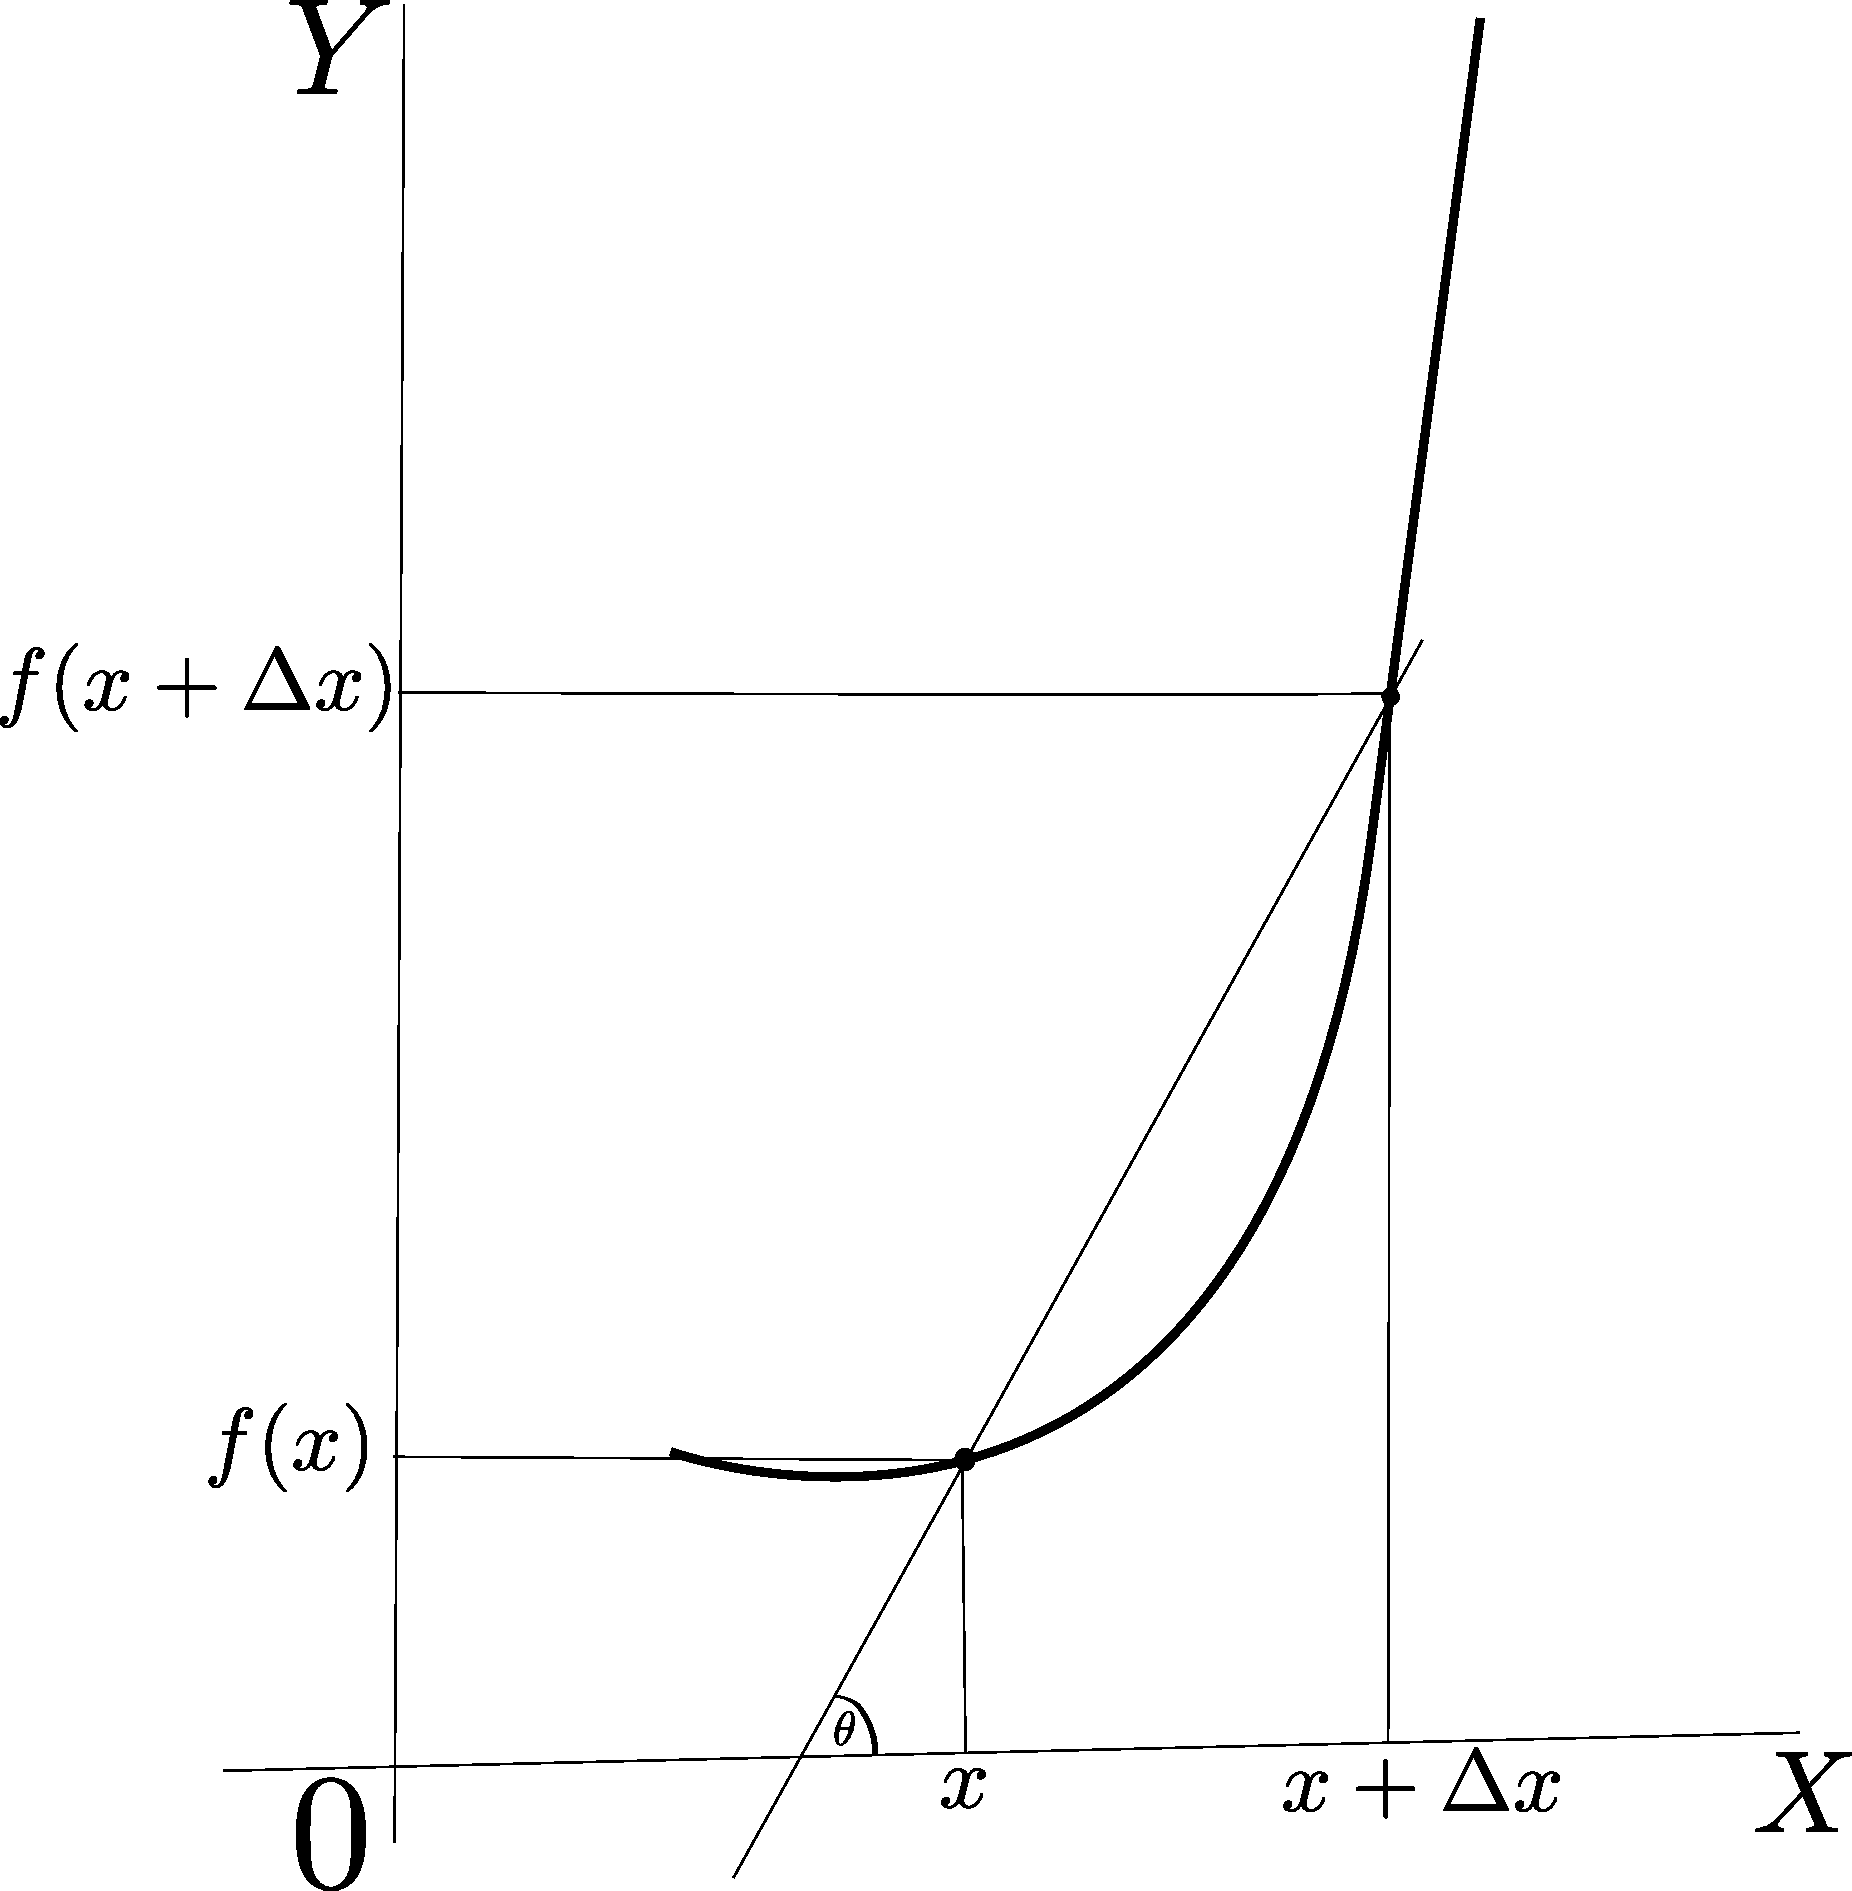
\includegraphics[scale=0.25]{figures/derivative-1.pdf}
	\caption{Understanding the derivative of a function as the slope of the secant line going through the two points on the function $(x,f(x))$ and $((x+\Delta x),f(x+\Delta x))$.\label{fig:derivative-1}}
\end{figure}
Let's take a look at Figure \ref{fig:derivative-1}. The slope of the line connecting two points $(x,f(x))$ and $( (x+\Delta x),f(x+\Delta x))$ is:
\begin{equation}
\nonumber \text{tan}(\theta) = m = \dfrac{\text{change in $y$}}{\text{change in $x$}} = \dfrac{f(x+\Delta x) - f(x)}{(x+\Delta x)-x} = \dfrac{f(x+\Delta x) - f(x)}{(\Delta x)} 
\end{equation}
But, the derivative tends to find the slope of the function (i.e., the rate of change of the function in y) on a given point in $x$, unlike the two given points in the example above. How can we accomplish that? 

We can find that value using the concept of limits. That is, we shrink the small difference $\Delta x$ towards 0 (Equation \ref{eqn:derivative-1}). It's that simple! Thus, the derivative at a point $x$ of a function $f(x)$ is the slope of the function at that point $x$ (Figure \ref{fig:derivative-2}).
\begin{figure}[!th]
	\centering
	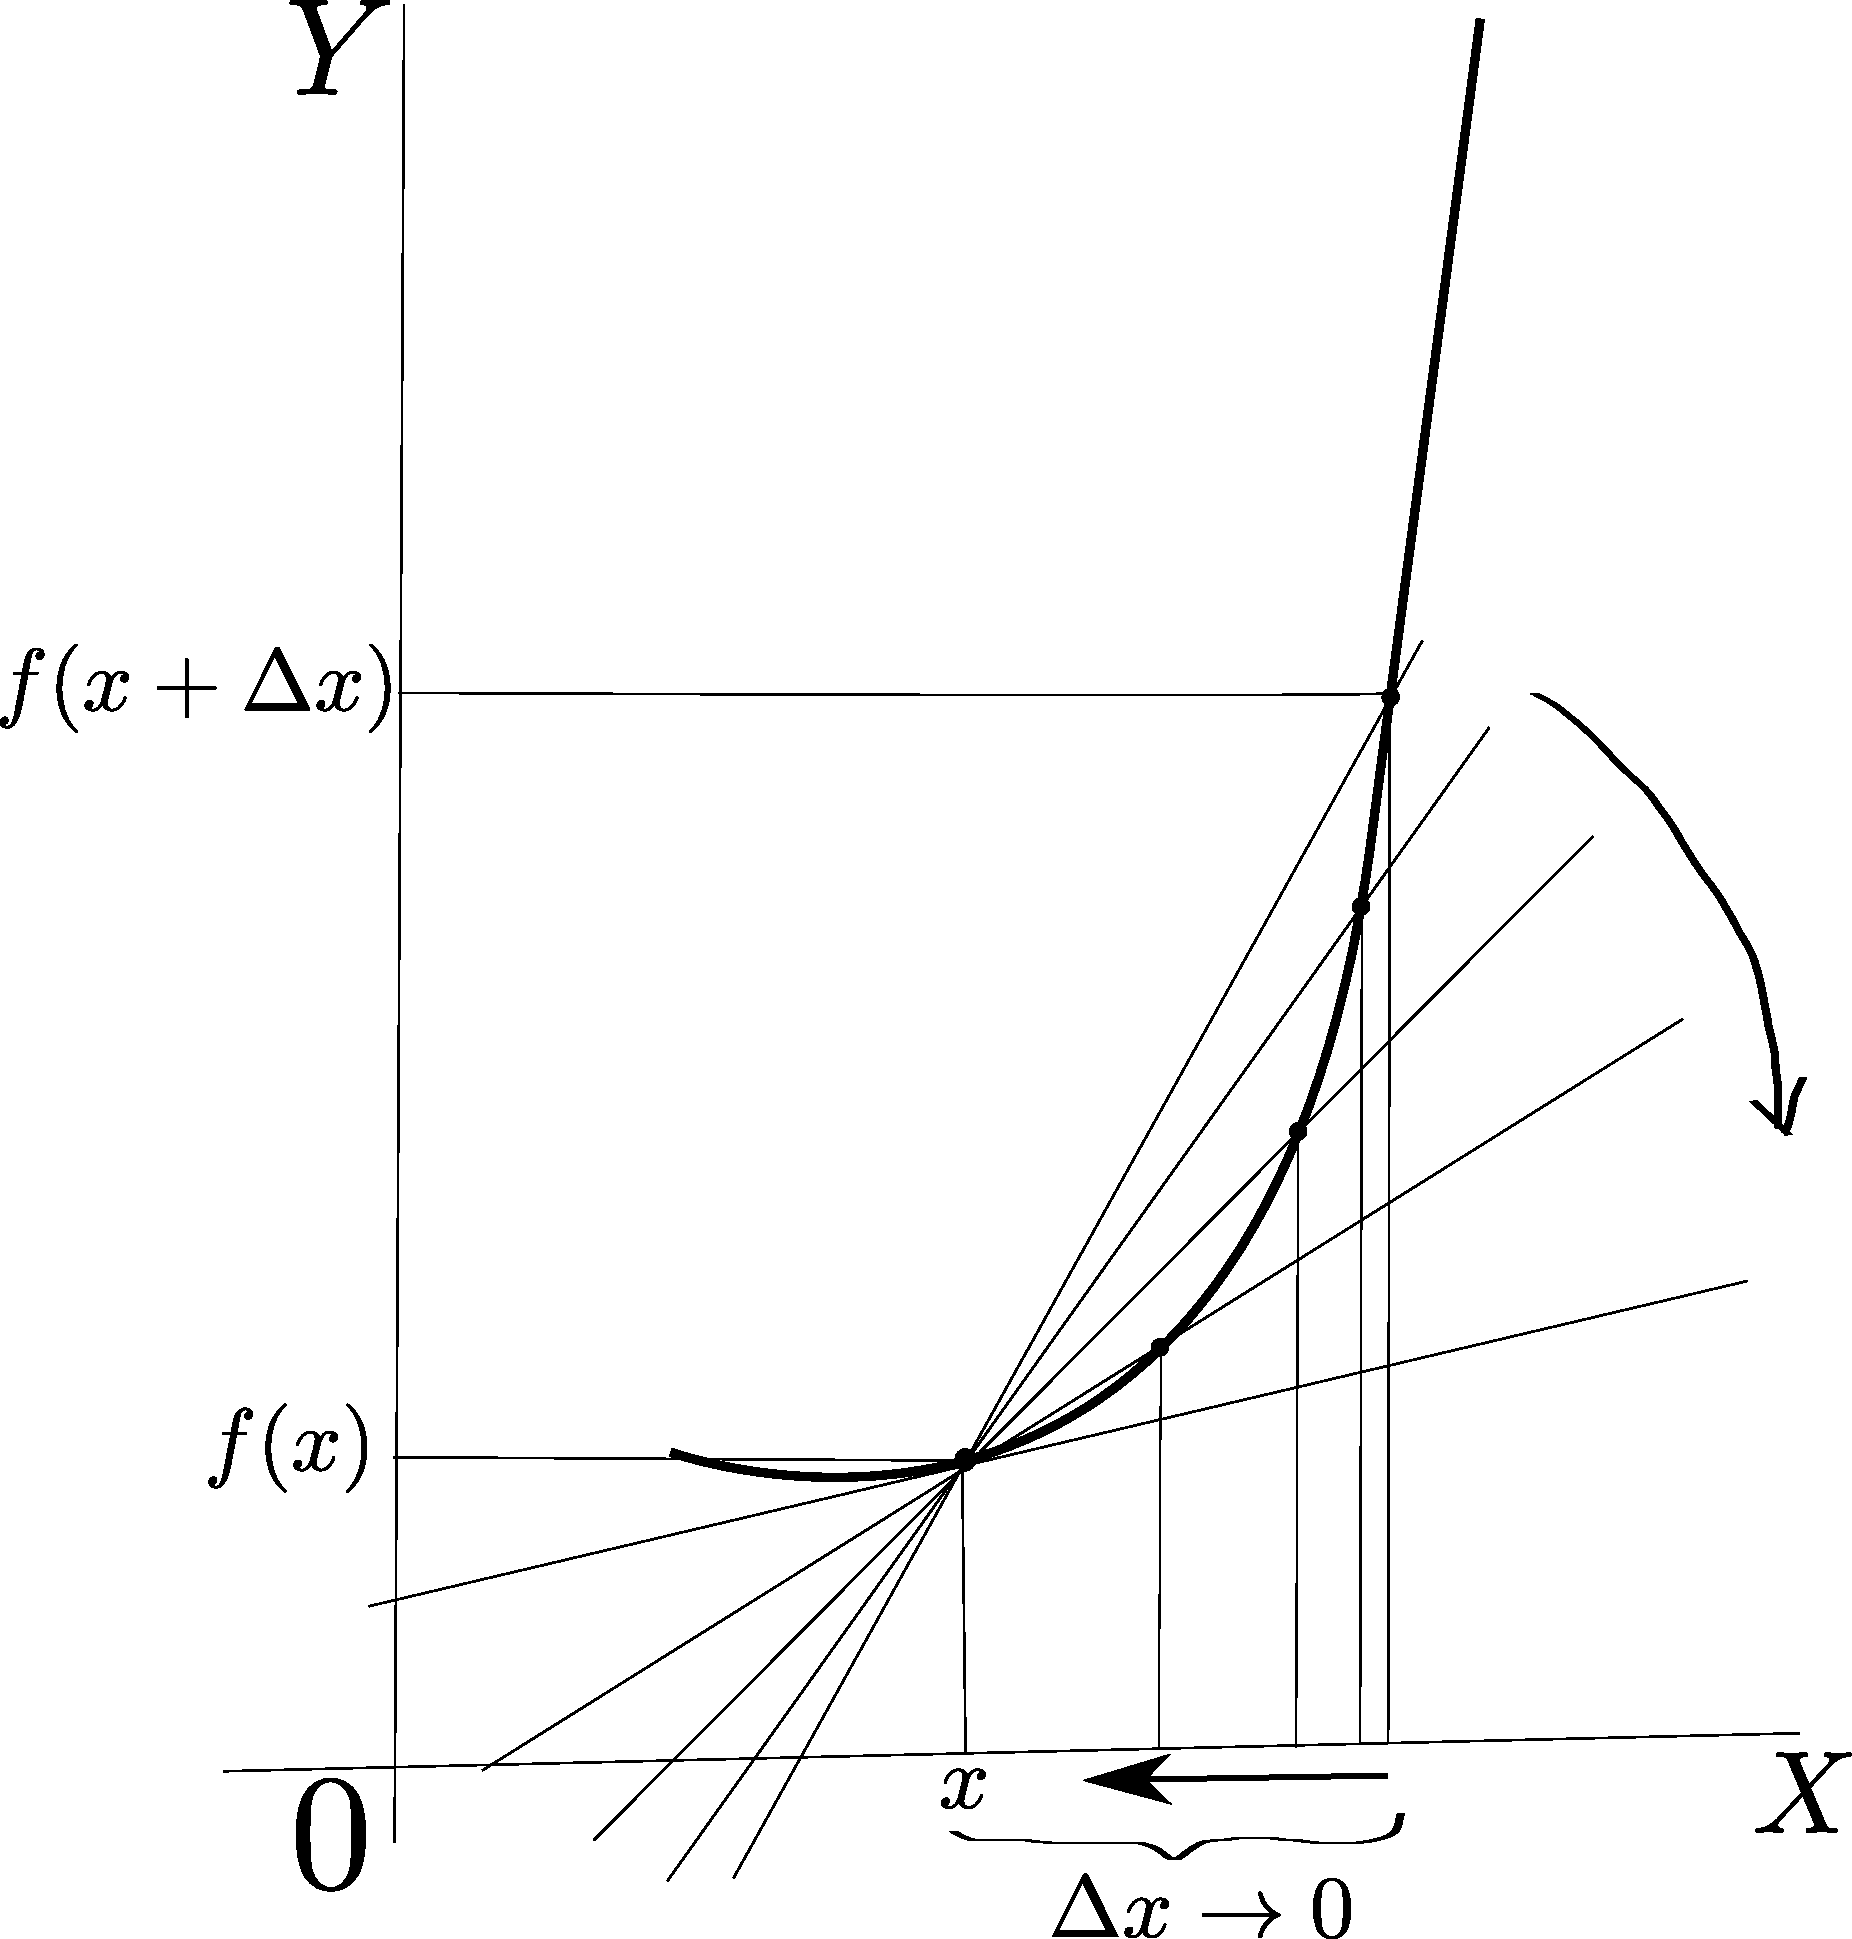
\includegraphics[scale=0.25]{figures/derivative-2.pdf}
	\caption{Deriviative is the slope of the function $f(x)$ at point $x$.\label{fig:derivative-2}}
\end{figure}

More intuitive explanations about the derivative can be found in MathIsFun blog\cite{introduction_to_derivatives} and the Khalid Azad's blog\cite{intuition_for_the_derivative}.

Example 1:  What is $\dfrac{d}{dx} x^3$? In other words, let's say, $f(x) = x^3$, then what is $f'(x)$?

\begin{eqnarray}
	\nonumber f'(x) &=& \lim_{\Delta x\rightarrow 0}\dfrac{f(x+\Delta x) - f(x)}{\Delta x}\\
	\nonumber &=& \lim_{\Delta x\rightarrow 0}\dfrac{(x+\Delta x)^3 - x^3}{\Delta x}\\
	\nonumber &=& \lim_{\Delta x\rightarrow 0}\dfrac{\cancel{x^3}+3x^2\Delta x+3x\Delta x^2+\Delta x^3 - \cancel{x^3}}{\Delta x}\\
	\nonumber &=& \lim_{\Delta x\rightarrow 0}3x^2+3x\Delta x+\Delta x^2\\
	\nonumber &=& 3x^2 + 0 + 0\\
	\nonumber &=& 3x^2
\end{eqnarray}
\textbf{The first and the second derivatives }\cite{opencalc2}: The first derivative of the function $f(x)$, which is $f'(x)$ or $\dfrac{df}{dx}$, is the slope of the tangent line to the function at the point $x$. Essentially, the first derivative tells us whether a function is increasing or decreasing, and by how much it is increasing or decreasing in terms of slope. A positive slope tells us that as $x$ increases, $f(x)$ also increases. Negative slope tells us that, as $x$ increases, $f(x)$ decreases. However, a zero slope does not tell us anthing in particular: the function may be increasing, decreasing, or at a local maximum or a local minimum at that point. So, we find:
\begin{itemize}
	\item if $f'(p) = \left.\dfrac{df}{dx}\right|_{x=p} > 0$, then $f(x)$ is an increasing function at $x=p$.
	\item if $f'(p) = \left.\dfrac{df}{dx}\right|_{x=p} < 0$, then $f(x)$ is a decreasing function at $x=p$.
	\item if $f'(p) = \left.\dfrac{df}{dx}\right|_{x=p} = 0$, then $f(x)$ is at critical point at $x=p$. We do not know anything new about the behavior of $f(x)$ at $x=p$.
\end{itemize}

If $f(x)$ is differentiable at point $p$ and $f'(p)=0=\text{tan}\theta$ (i.e., the tangent is parallel to $X$ axis, Figure \ref{fig:derivative-3}), then we call $p$ a critical point or stationary point of $f(x)$. A point $p$ at which the derivative of $f(x)$ is not defined is called a singular point of $f(x)$.
\begin{figure}[!h]
	\centering
	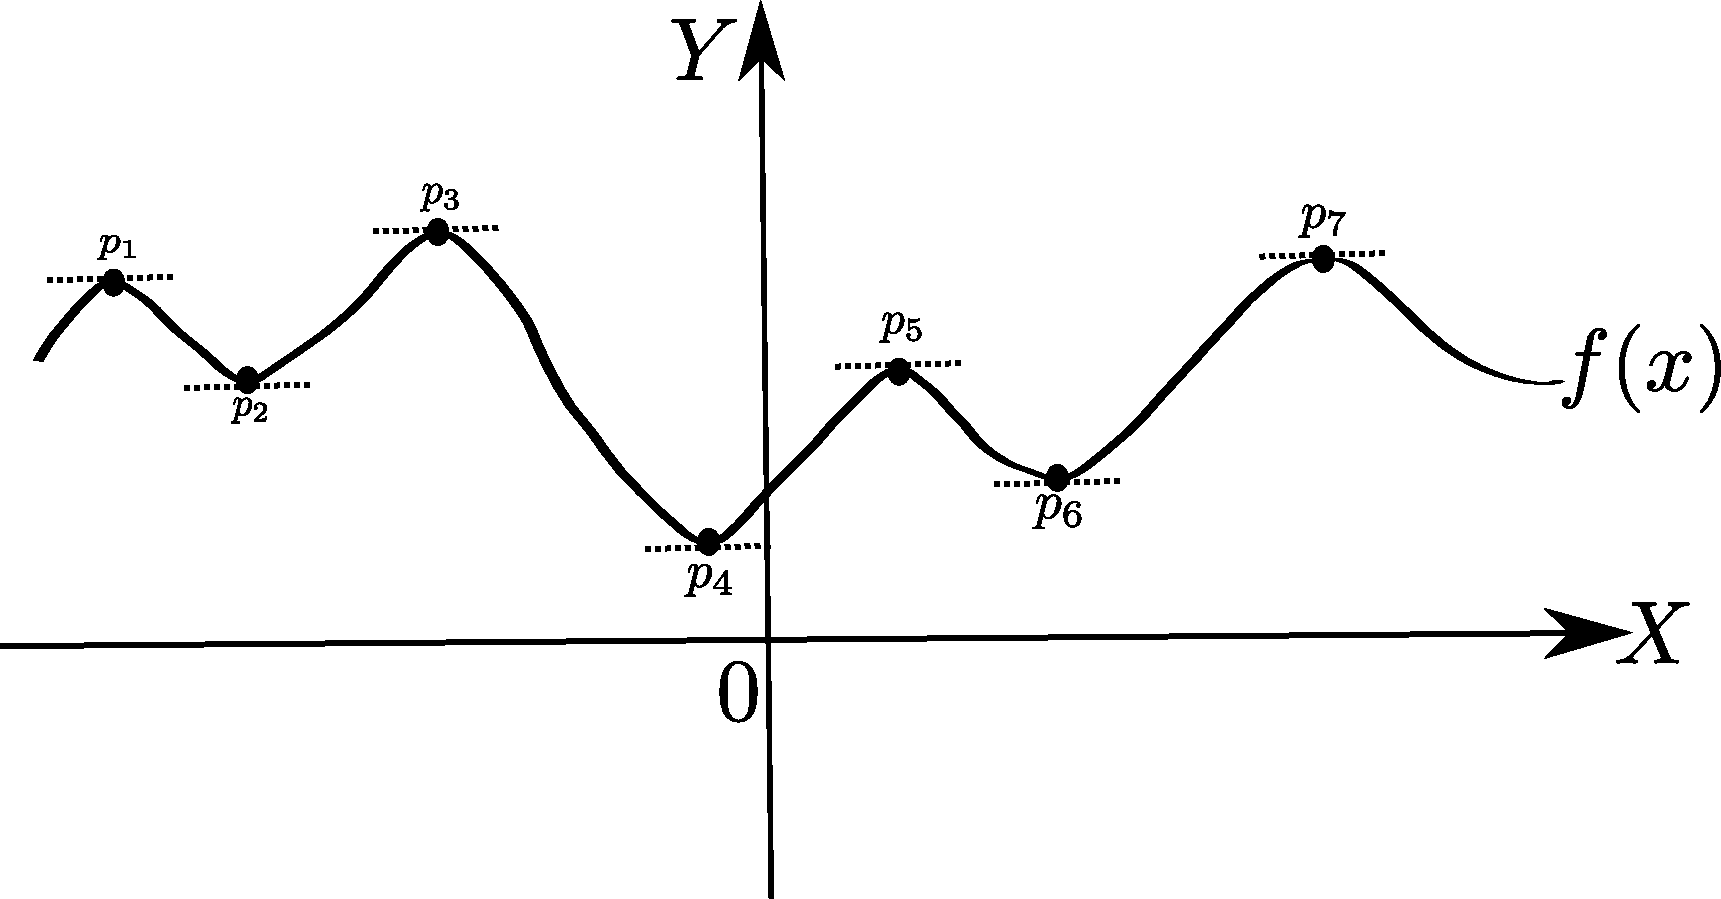
\includegraphics[scale=0.5]{figures/derivative-3.pdf}
	\caption{The plot of a function $f(x)$. The first derivatives of the function at points $p_1, p_2, p_3, p_4, p_5, p_6, p_7$ are zero; we see that the tangent lines on these points have slope 0, i.e., are parallel to the $X$ axis, $\text{tan}\theta = \left.\dfrac{df}{dx}\right|_{x=p_i} = 0$, for $i=1\cdots 7$. So, these 7 points are called the critical points of the function. We can't say anything further than this phenomenon whether the critical points are either local minimum, or local maximum by looking at the critical points alone. That's why we need the second derivative test.\label{fig:derivative-3}}
\end{figure}

 The second derivative of a function is the derivative of the derivative of that function. We write it as $f''(x)$ or $\dfrac{d^2f}{dx^2}$. While the first derivative can tell us if the function is increasing or decreasing, the second derivative tells us if the first derivative is increasing or decreasing, i.e., the slope of the tangent line to the function is increasing or decreasing. If the second derivative is positive, then the first derivative is increasing, so that the slope of the tangent line to the function is increasing as $x$ increases. We see this phenomenon graphically as the curve of the graph being concave up. Likewise, if the second derivative is negative, then the first derivative is decreasing, so that the slope of the tangent line to the function is decreasing as $x$ increases. Graphically, we see this as the curve of the graph being concave down. At the points where the second derivative is zero, we do not learn anything about the shape of the graph: it may be concave up or concave down, or it may be changing from concave up to concave down or changing from concave down to concave up. So, let's summarize these:
 \begin{itemize}
 	\item if $\left.\dfrac{d^2f}{dx^2}\right|_{x=p} > 0$ at $x=p$, then the function $f(x)$ is concave up at $x=p$.
 	\item if $\left. \dfrac{d^2f}{dx^2}\right|_{x=p} < 0$ at $x=p$, then $f(x)$ is concave down at $x=p$.
 	\item if $\left. \dfrac{d^2f}{dx^2}\right|_{x=p} = 0$ at $x=p$, then we do not know anything new about the behavior of $f(x)$ at $x=p$.
 \end{itemize}
 
 \textbf{Critical Points and the second derivative test:} We learned that, when $x$ is a critical point of the function $f(x)$, we do not learn anything new about the function at that point: it could be increasing, decreasing, a local minimum or a local maximum. We can often use the second derivative of the function, to find out when $x$ is a local maximum or a local minimum.
 
 \textbf{Case 1:} Recall that $x$ is a critical point of a function when the slope of the function is zero at that point. Now, suppose that $x$ is a critical point and the second derivative of the function at that point is positive. The positive second derivative at $x$ tells us that the derivative of $f(x)$ is increasing at that point and, graphically, that the curve of the graph is concave up at that point. The only way to sketch the graph of a function at a point where the slope of the function is zero but the graph is concave up is to make that point a local minimum of the function. So, if $x$ is a critical point of $f(x)$ and the second derivative of $f(x)$ is positive, then $x$ is a local minimum of $f(x)$.
 
 \textbf{Case 2:} If $x$ is a critical point of $f(x)$, and the second deriviative of $f(x)$ is negative, then the slope of the graph of the function is zero at that point, but the curve of the graph is concave down. The only way to draw a graph like this is to make the point $x$ a local maximum of the function. Hence, we get that if $x$ is a critical point of $f(x)$ and the second derivative of $f(x)$ is negative, then $x$ is a local maximum of $f(x)$.
 
 \textbf{Case 3:} If $x$ is a critical point of $f(x)$ and the second derivative is zero, then we learn no new information about that point. The point $x$ may be a local maximum or a local minimum, and the function may also be increasing or decreasing at that point.
 
 Thus, in a summary:
 \begin{itemize}
 	\item If $\left.\dfrac{df}{dx}\right|_{x=p} = 0$ and $\left. \dfrac{d^2f}{dx^2}\right|_{x=p} > 0$, then $f(x)$ has a local minimum at $x=p$.
 	\item If $\left.\dfrac{df}{dx}\right|_{x=p} = 0$ and $\left. \dfrac{d^2f}{dx^2}\right|_{x=p} < 0$, then $f(x)$ has a local maximum at $x=p$.
 	\item If $\left.\dfrac{df}{dx}\right|_{x=p} = 0$ and $\left. \dfrac{d^2f}{dx^2}\right|_{x=p} = 0$, then we learn no new information about the behavior of $f(x)$ at $x=p$.
 \end{itemize}
 
 Example 2: Given $f(x) = x^3 - 9x^2 + 15x - 7$, find critical points of $f(x)$ and check if any of the points are local maximum or local minimum.

 Ans: The derivative of $f(x)$ is $f'(x) = 3x^2 - 18x + 15$. We need to solve for $x$ if $f'(x)=0$. That is,
 \begin{eqnarray}
 \nonumber f'(x) &=& 0\\
 \nonumber 3x^2-18x+15 &=& 0\\
 \nonumber x^2 - 6x + 5 &=& 0\\
 \nonumber x^2 - x - 5x + 5 &=& 0\\
 \nonumber x(x-1) - 5(x-1) &=& 0\\
 \nonumber (x-1)(x-5) &=& 0\\
 \nonumber x = \text{1 or 5}
 \end{eqnarray}

 So, $f(x)$ has critical points at $x=1$ and $x=5$. We now apply the second derivative test: $f''(x) = 6x-18$. Then we put the critical points on the $f''(x)$ for the local minimum/maximum test:
 
 At $x=1$, $f''(1) = 6.1-18=-12 < 0$, so the critical point $x=1$ is the local maximum of the function $f(x)$.
 
 At $x=5$, $f''(5) = 6.5-18=12 > 0$, thus the critical point $x=5$ is the local minimum of the function $f(x)$.
\section{Partial Derivative}
\label{term:partial_derivative}
A partial derivative of a function of several variables is its derivative with respect to one of those variables, with the others held constant\cite{wiki:PartialDerivative}\cite{khan:PartialDerivative}.

Let's assume $z = f(x,y)$, represents a surface in 3D Euclidean space (Figure \ref{fig:partial-derivative-1}).
\begin{figure}[!h]
	\centering
	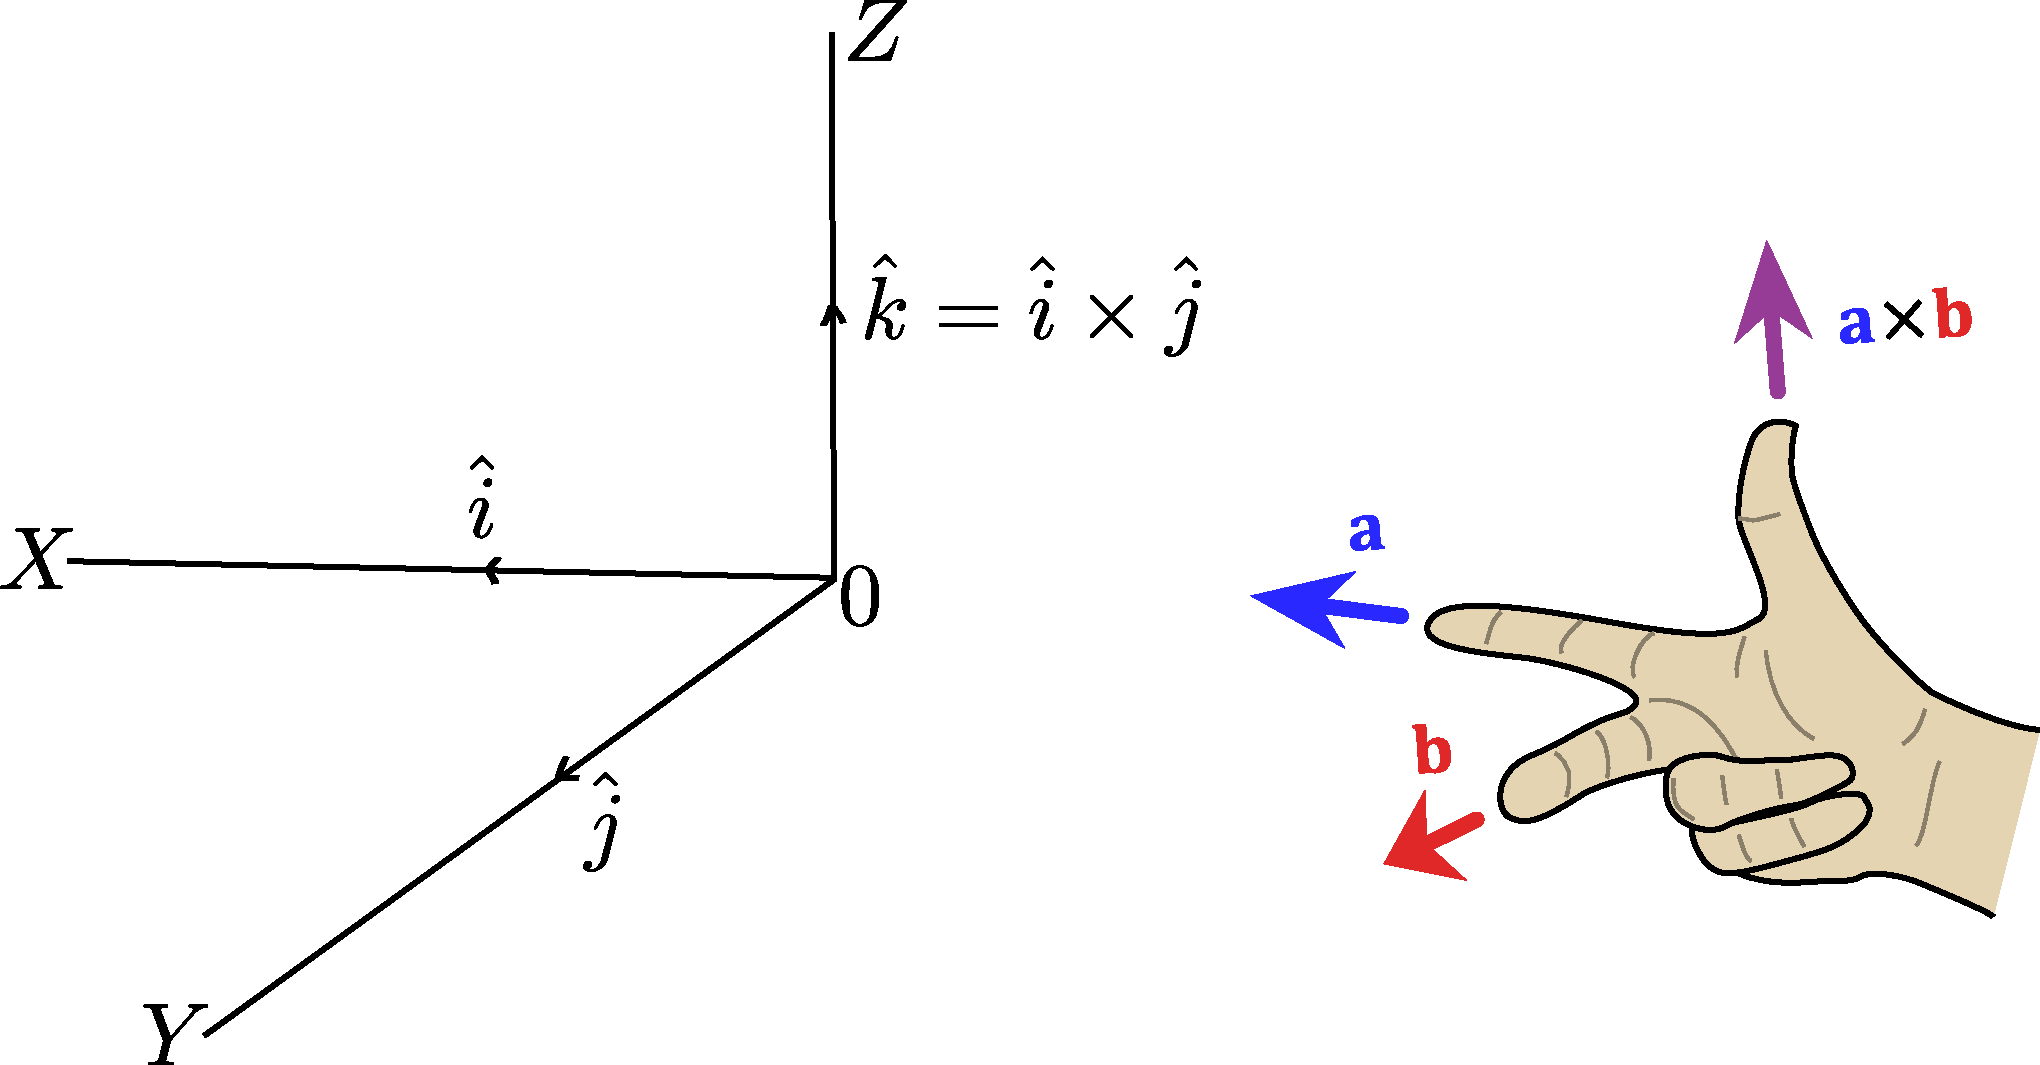
\includegraphics[scale=0.5]{figures/partial-derivative-1.pdf}
	\caption{Visualizing the 3D Euclidean space using the right hand rule. The unit vector acros the $Z$ axis, $\hat{k}$ is equal to the cross product of the unit vectors across the $X$ and $Y$ axes, $\hat{i}$ and $\hat{j}$ respectively. That is, $\hat{k} = \hat{i}\times \hat{j}$\label{fig:partial-derivative-1}}
\end{figure}

\begin{knitrout}
\definecolor{shadecolor}{rgb}{0.969, 0.969, 0.969}\color{fgcolor}\begin{kframe}
\begin{alltt}
\hlcom{#Let's plot the function z = f(x,y) = x^2 + xy + y^2}
\hlstd{x} \hlkwb{<-} \hlkwd{seq}\hlstd{(}\hlopt{-}\hlnum{10}\hlstd{,}\hlnum{10}\hlstd{,}\hlkwc{length}\hlstd{=}\hlnum{30}\hlstd{)} \hlcom{#generate equally spaced 30 points }
                \hlcom{#on the X axis (between -10 and 10)}
\hlstd{y} \hlkwb{<-} \hlstd{x} \hlcom{#use the same 30 points for Y axis}

\hlstd{f} \hlkwb{<-} \hlkwa{function}\hlstd{(}\hlkwc{x}\hlstd{,}\hlkwc{y}\hlstd{)\{ r} \hlkwb{<-} \hlstd{x}\hlopt{^}\hlnum{2}\hlopt{+}\hlstd{x}\hlopt{*}\hlstd{y}\hlopt{+}\hlstd{y}\hlopt{^}\hlnum{2}\hlstd{\}} \hlcom{#define the function here}
\hlstd{z} \hlkwb{<-} \hlkwd{outer}\hlstd{(x,y,f)} \hlcom{#outer product of the x vector and y vector. }
                \hlcom{#Instead of product, the outer function will apply }
                \hlcom{#the f() function to get the value for z's}

\hlcom{#now we can plot the surface}
\hlcom{#op <- par(bg = 'white') #white background}
\hlcom{#theta & phi control the viewing angle}
        \hlcom{#theta moves the viewing angle left and right}
        \hlcom{#phi moves it up and down}
\hlkwd{par}\hlstd{(}\hlkwc{mfrow}\hlstd{=}\hlkwd{c}\hlstd{(}\hlnum{2}\hlstd{,}\hlnum{2}\hlstd{))}
\hlkwd{persp}\hlstd{(x,y,z,}\hlkwc{theta}\hlstd{=}\hlnum{40}\hlstd{,}\hlkwc{phi}\hlstd{=}\hlopt{-}\hlnum{20}\hlstd{,}\hlkwc{col}\hlstd{=}\hlstr{"lightblue"}\hlstd{)}
\hlkwd{persp}\hlstd{(x,y,z,}\hlkwc{theta}\hlstd{=}\hlopt{-}\hlnum{40}\hlstd{,}\hlkwc{phi}\hlstd{=}\hlnum{20}\hlstd{,}\hlkwc{col}\hlstd{=}\hlstr{"lightblue"}\hlstd{)}
\hlkwd{persp}\hlstd{(x,y,z,}\hlkwc{theta}\hlstd{=}\hlopt{-}\hlnum{30}\hlstd{,}\hlkwc{phi}\hlstd{=}\hlopt{-}\hlnum{30}\hlstd{,}\hlkwc{col}\hlstd{=}\hlstr{"lightblue"}\hlstd{)}
\hlkwd{persp}\hlstd{(x,y,z,}\hlkwc{theta}\hlstd{=}\hlopt{-}\hlnum{30}\hlstd{,}\hlkwc{phi}\hlstd{=}\hlnum{30}\hlstd{,}\hlkwc{col}\hlstd{=}\hlstr{"lightblue"}\hlstd{)}
\end{alltt}
\end{kframe}

{\centering 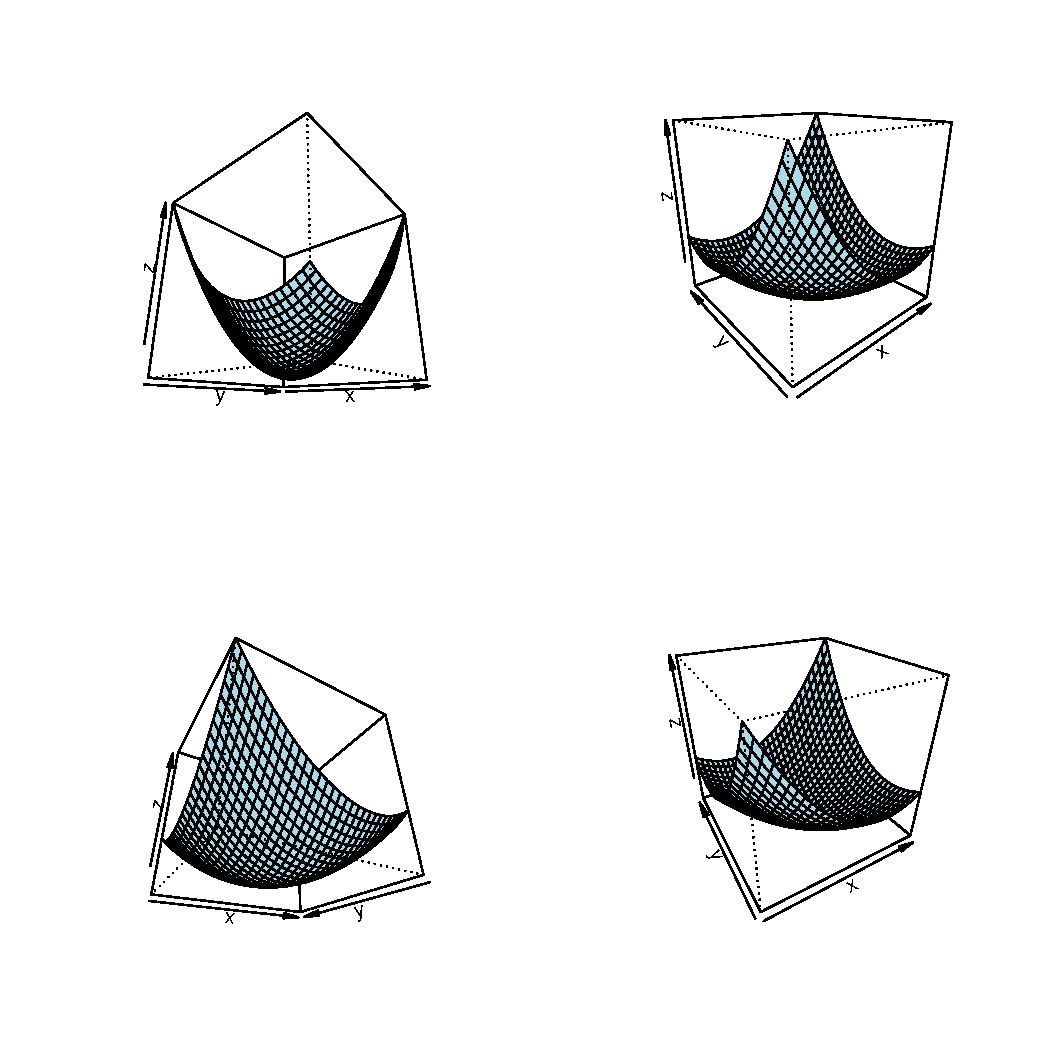
\includegraphics[width=6in]{figure/minimal-Plot-surface-1-1} 

}



\end{knitrout}

With the function $z=x^2+xy+y^2$, the first derivative with respect to $x$ by holding $y$ constant, we get:
\begin{eqnarray}
\nonumber \dfrac{\partial z}{\partial x} = 2x+y
\end{eqnarray}
Then, we have an intersecting plane for the 3D plot of the $z$ function, for instance $y=1$. Then at the intersection of the plane and the surface plot, we have a curve, and the slope to that curve is the partial derivative of $z$ with respect to $x$ by holding $y$ constant.
\begin{knitrout}
\definecolor{shadecolor}{rgb}{0.969, 0.969, 0.969}\color{fgcolor}\begin{kframe}
\begin{alltt}
\hlcom{#Let's plot the function z = f(x,y) = x^2 + xy + y^2}
\hlstd{x} \hlkwb{<-} \hlkwd{seq}\hlstd{(}\hlopt{-}\hlnum{10}\hlstd{,}\hlnum{10}\hlstd{,}\hlkwc{length}\hlstd{=}\hlnum{30}\hlstd{)} \hlcom{#generate equally spaced 30 points }
                \hlcom{#on the X axis (between -10 and 10)}
\hlstd{y} \hlkwb{<-} \hlstd{x} \hlcom{#use the same 30 points for Y axis}

\hlstd{f} \hlkwb{<-} \hlkwa{function}\hlstd{(}\hlkwc{x}\hlstd{,}\hlkwc{y}\hlstd{)\{}
        \hlstd{r} \hlkwb{<-} \hlstd{x}\hlopt{^}\hlnum{2}\hlopt{+}\hlstd{x}\hlopt{*}\hlstd{y}\hlopt{+}\hlstd{y}\hlopt{^}\hlnum{2}
\hlstd{\}} \hlcom{#define the function here}
\hlstd{z} \hlkwb{<-} \hlkwd{outer}\hlstd{(x,y,f)} \hlcom{#outer product of the x vector and y vector. }
                \hlcom{#Instead of product, the outer function will apply }
                \hlcom{#the f() function to get the value for z's}

\hlstd{res} \hlkwb{<-} \hlkwd{persp}\hlstd{(x,y,z,}\hlkwc{phi}\hlstd{=}\hlopt{-}\hlnum{20}\hlstd{,}\hlkwc{col}\hlstd{=}\hlstr{"lightblue"}\hlstd{,}
        \hlkwc{main}\hlstd{=}\hlstr{"The surface plot of z with an intersecting plane with holding y=1"}\hlstd{)}
\hlkwd{polygon}\hlstd{(}\hlkwd{trans3d}\hlstd{(}\hlkwd{c}\hlstd{(}\hlopt{-}\hlnum{10}\hlstd{,}\hlnum{10}\hlstd{,}\hlnum{10}\hlstd{,}\hlopt{-}\hlnum{10}\hlstd{,}\hlopt{-}\hlnum{10}\hlstd{),} \hlkwd{c}\hlstd{(}\hlnum{1}\hlstd{,}\hlnum{1}\hlstd{,}\hlnum{1}\hlstd{,}\hlnum{1}\hlstd{,}\hlnum{1}\hlstd{),}\hlkwd{c}\hlstd{(}\hlnum{0}\hlstd{,}\hlnum{0}\hlstd{,}\hlnum{300}\hlstd{,}\hlnum{300}\hlstd{,}\hlnum{0}\hlstd{),res),}
                        \hlkwc{col}\hlstd{=}\hlkwd{rgb}\hlstd{(}\hlnum{1}\hlstd{,}\hlnum{0}\hlstd{,}\hlnum{0}\hlstd{,}\hlnum{0.2}\hlstd{),}\hlkwc{border}\hlstd{=}\hlnum{NA}\hlstd{)}
\end{alltt}
\end{kframe}

{\centering 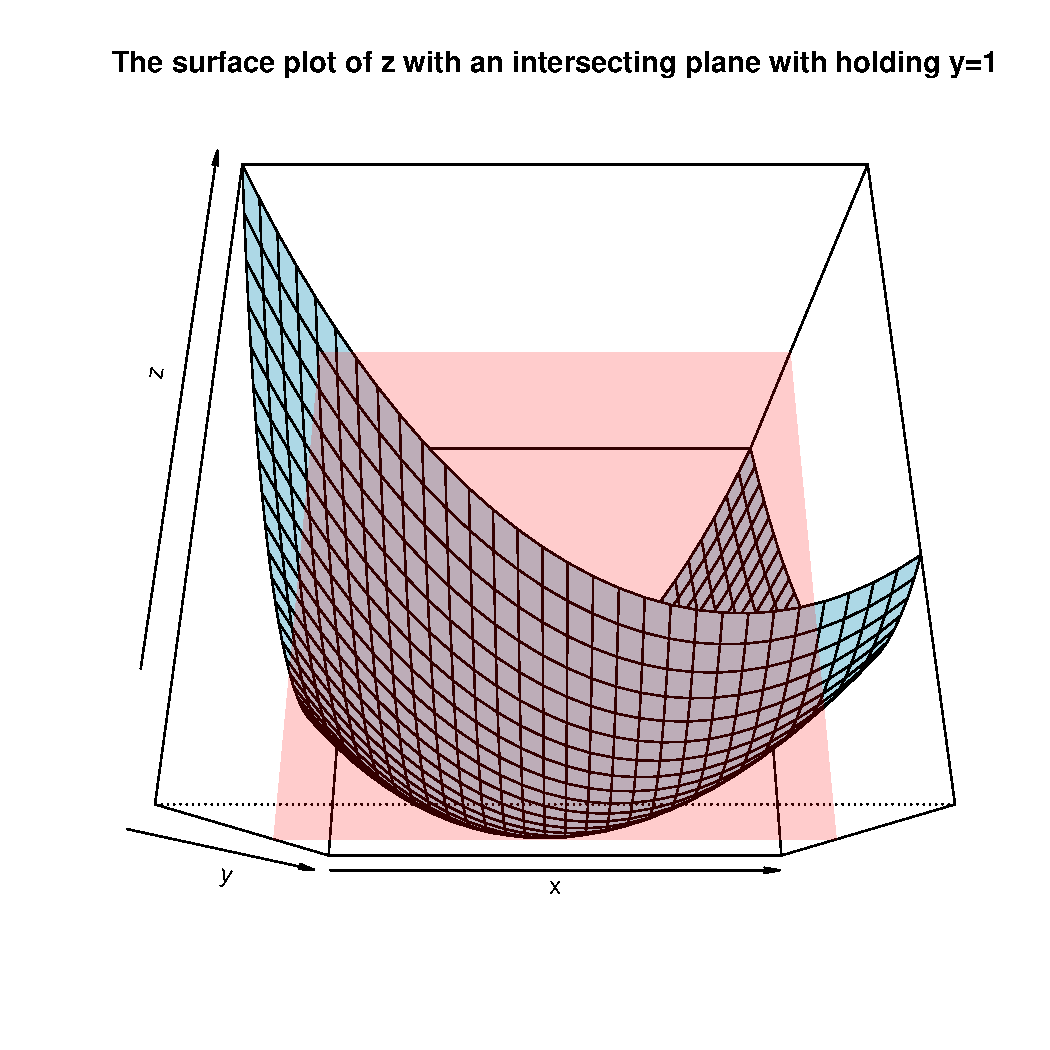
\includegraphics[width=3in]{figure/minimal-Plot-surface-2-1} 

}



\end{knitrout}


Similarly, the first derivative of $z$ with respect to $y$ would be:
\begin{eqnarray}
\nonumber \dfrac{\partial z}{\partial y} = x+2y
\end{eqnarray}
\begin{knitrout}
\definecolor{shadecolor}{rgb}{0.969, 0.969, 0.969}\color{fgcolor}\begin{kframe}
\begin{alltt}
\hlcom{#Let's plot the function z = f(x,y) = x^2 + xy + y^2}
\hlstd{x} \hlkwb{<-} \hlkwd{seq}\hlstd{(}\hlopt{-}\hlnum{10}\hlstd{,}\hlnum{10}\hlstd{,}\hlkwc{length}\hlstd{=}\hlnum{30}\hlstd{)} \hlcom{#generate equally spaced 30 points }
                \hlcom{#on the X axis (between -10 and 10)}
\hlstd{y} \hlkwb{<-} \hlstd{x} \hlcom{#use the same 30 points for Y axis}

\hlstd{f} \hlkwb{<-} \hlkwa{function}\hlstd{(}\hlkwc{x}\hlstd{,}\hlkwc{y}\hlstd{)\{}
        \hlstd{r} \hlkwb{<-} \hlstd{x}\hlopt{^}\hlnum{2}\hlopt{+}\hlstd{x}\hlopt{*}\hlstd{y}\hlopt{+}\hlstd{y}\hlopt{^}\hlnum{2}
\hlstd{\}} \hlcom{#define the function here}
\hlstd{z} \hlkwb{<-} \hlkwd{outer}\hlstd{(x,y,f)} \hlcom{#outer product of the x vector and y vector. }
                \hlcom{#Instead of product, the outer function will apply }
                \hlcom{#the f() function to get the value for z's}

\hlstd{res} \hlkwb{<-} \hlkwd{persp}\hlstd{(x,y,z,}\hlkwc{theta}\hlstd{=}\hlopt{-}\hlnum{20}\hlstd{,}\hlkwc{phi}\hlstd{=}\hlopt{-}\hlnum{40}\hlstd{,}\hlkwc{col}\hlstd{=}\hlstr{"lightblue"}\hlstd{,}
        \hlkwc{main}\hlstd{=}\hlstr{"The surface plot of z with an intersecting plane with holding x=1"}\hlstd{)}
\hlkwd{polygon}\hlstd{(}\hlkwd{trans3d}\hlstd{(}\hlkwd{c}\hlstd{(}\hlnum{1}\hlstd{,}\hlnum{1}\hlstd{,}\hlnum{1}\hlstd{,}\hlnum{1}\hlstd{,}\hlnum{1}\hlstd{),} \hlkwd{c}\hlstd{(}\hlopt{-}\hlnum{10}\hlstd{,}\hlnum{10}\hlstd{,}\hlnum{10}\hlstd{,}\hlopt{-}\hlnum{10}\hlstd{,}\hlopt{-}\hlnum{10}\hlstd{),}\hlkwd{c}\hlstd{(}\hlnum{0}\hlstd{,}\hlnum{0}\hlstd{,}\hlnum{300}\hlstd{,}\hlnum{300}\hlstd{,}\hlnum{0}\hlstd{),res),}
                        \hlkwc{col}\hlstd{=}\hlkwd{rgb}\hlstd{(}\hlnum{0}\hlstd{,}\hlnum{1}\hlstd{,}\hlnum{0}\hlstd{,}\hlnum{0.2}\hlstd{),}\hlkwc{border}\hlstd{=}\hlnum{NA}\hlstd{)}
\end{alltt}
\end{kframe}

{\centering 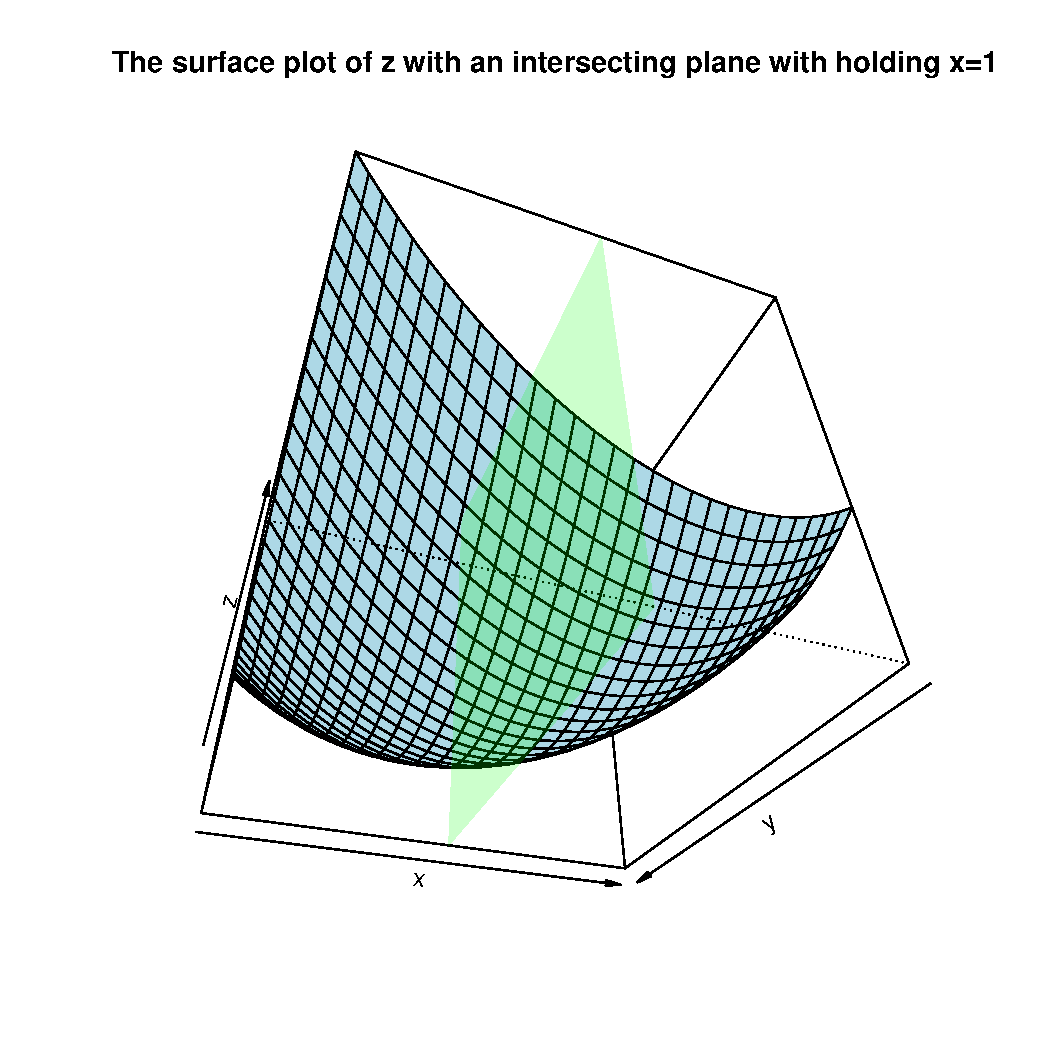
\includegraphics[width=3in]{figure/minimal-Plot-surface-3-1} 

}



\end{knitrout}

\section{Directional Derivative}
\label{term:directional_derivative}
Let the function $f(x,y)$ be the height of a mountain range at each point $\vec x=(x,y)$\cite{mathInsight:DirectionalDerivative} (Figure \ref{fig:directional_derivative_1}). If you stand at some point $\vec x=\vec a$, the slope of the ground in front of you will depend on the direction you are facing. It might slope steeply up in one direction, be relatively flat in another direction, and slope steeply down in yet another direction.

The partial derivatives of $f$ will give the slope $\frac{\partial f}{\partial x}$ in the positive $x$ direction and the slope $\frac{\partial f}{\partial y}$ in the positive $y$ direction. We can generalize the partial derivatives to calculate the slope in any direction. The result is called the directional derivative.
	
The first step in taking a directional derivative, is to specify the direction. One way to do this is with a vector $\vec u=(u_1,u_2)$ that points in the direction in which we want to compute the slope. For simplicity, we will insist that $\vec u$ is a unit vector. We write the directional derivative $f$ in the direction $\vec u$ at the point $\vec a$ as $D_{\vec u}f(\vec a)$. We could define it with a limit definition just as the ordinary derivative:
\begin{eqnarray}
\nonumber D_{\vec u}f(\vec a) = \lim_{h\rightarrow 0}\dfrac{f(\vec a+h\vec u)-f(\vec a)}{h}
\end{eqnarray}
$D_{\vec u}f(\vec a)$ is the slope of $f(\vec x)$ when standing at the point $\vec a$ and facing the direction given by $\vec u$. $D_{\vec u}f(\vec a)$ is a number. In fact, the directional derivative is the same as a partial derive if $\vec u$ points in the positive $x$ direction (or positive $y$ direction). For example, if $\vec u=(1,0)$, then $D_{\vec u}f(\vec a) = \frac{\partial f}{\partial x}(\vec a)$. Similarly if $\vec u=(0,1)$, then $D_{\vec u}f(\vec a) = \frac{\partial f}{\partial y}(\vec a)$
\begin{figure}[!h]
\centering
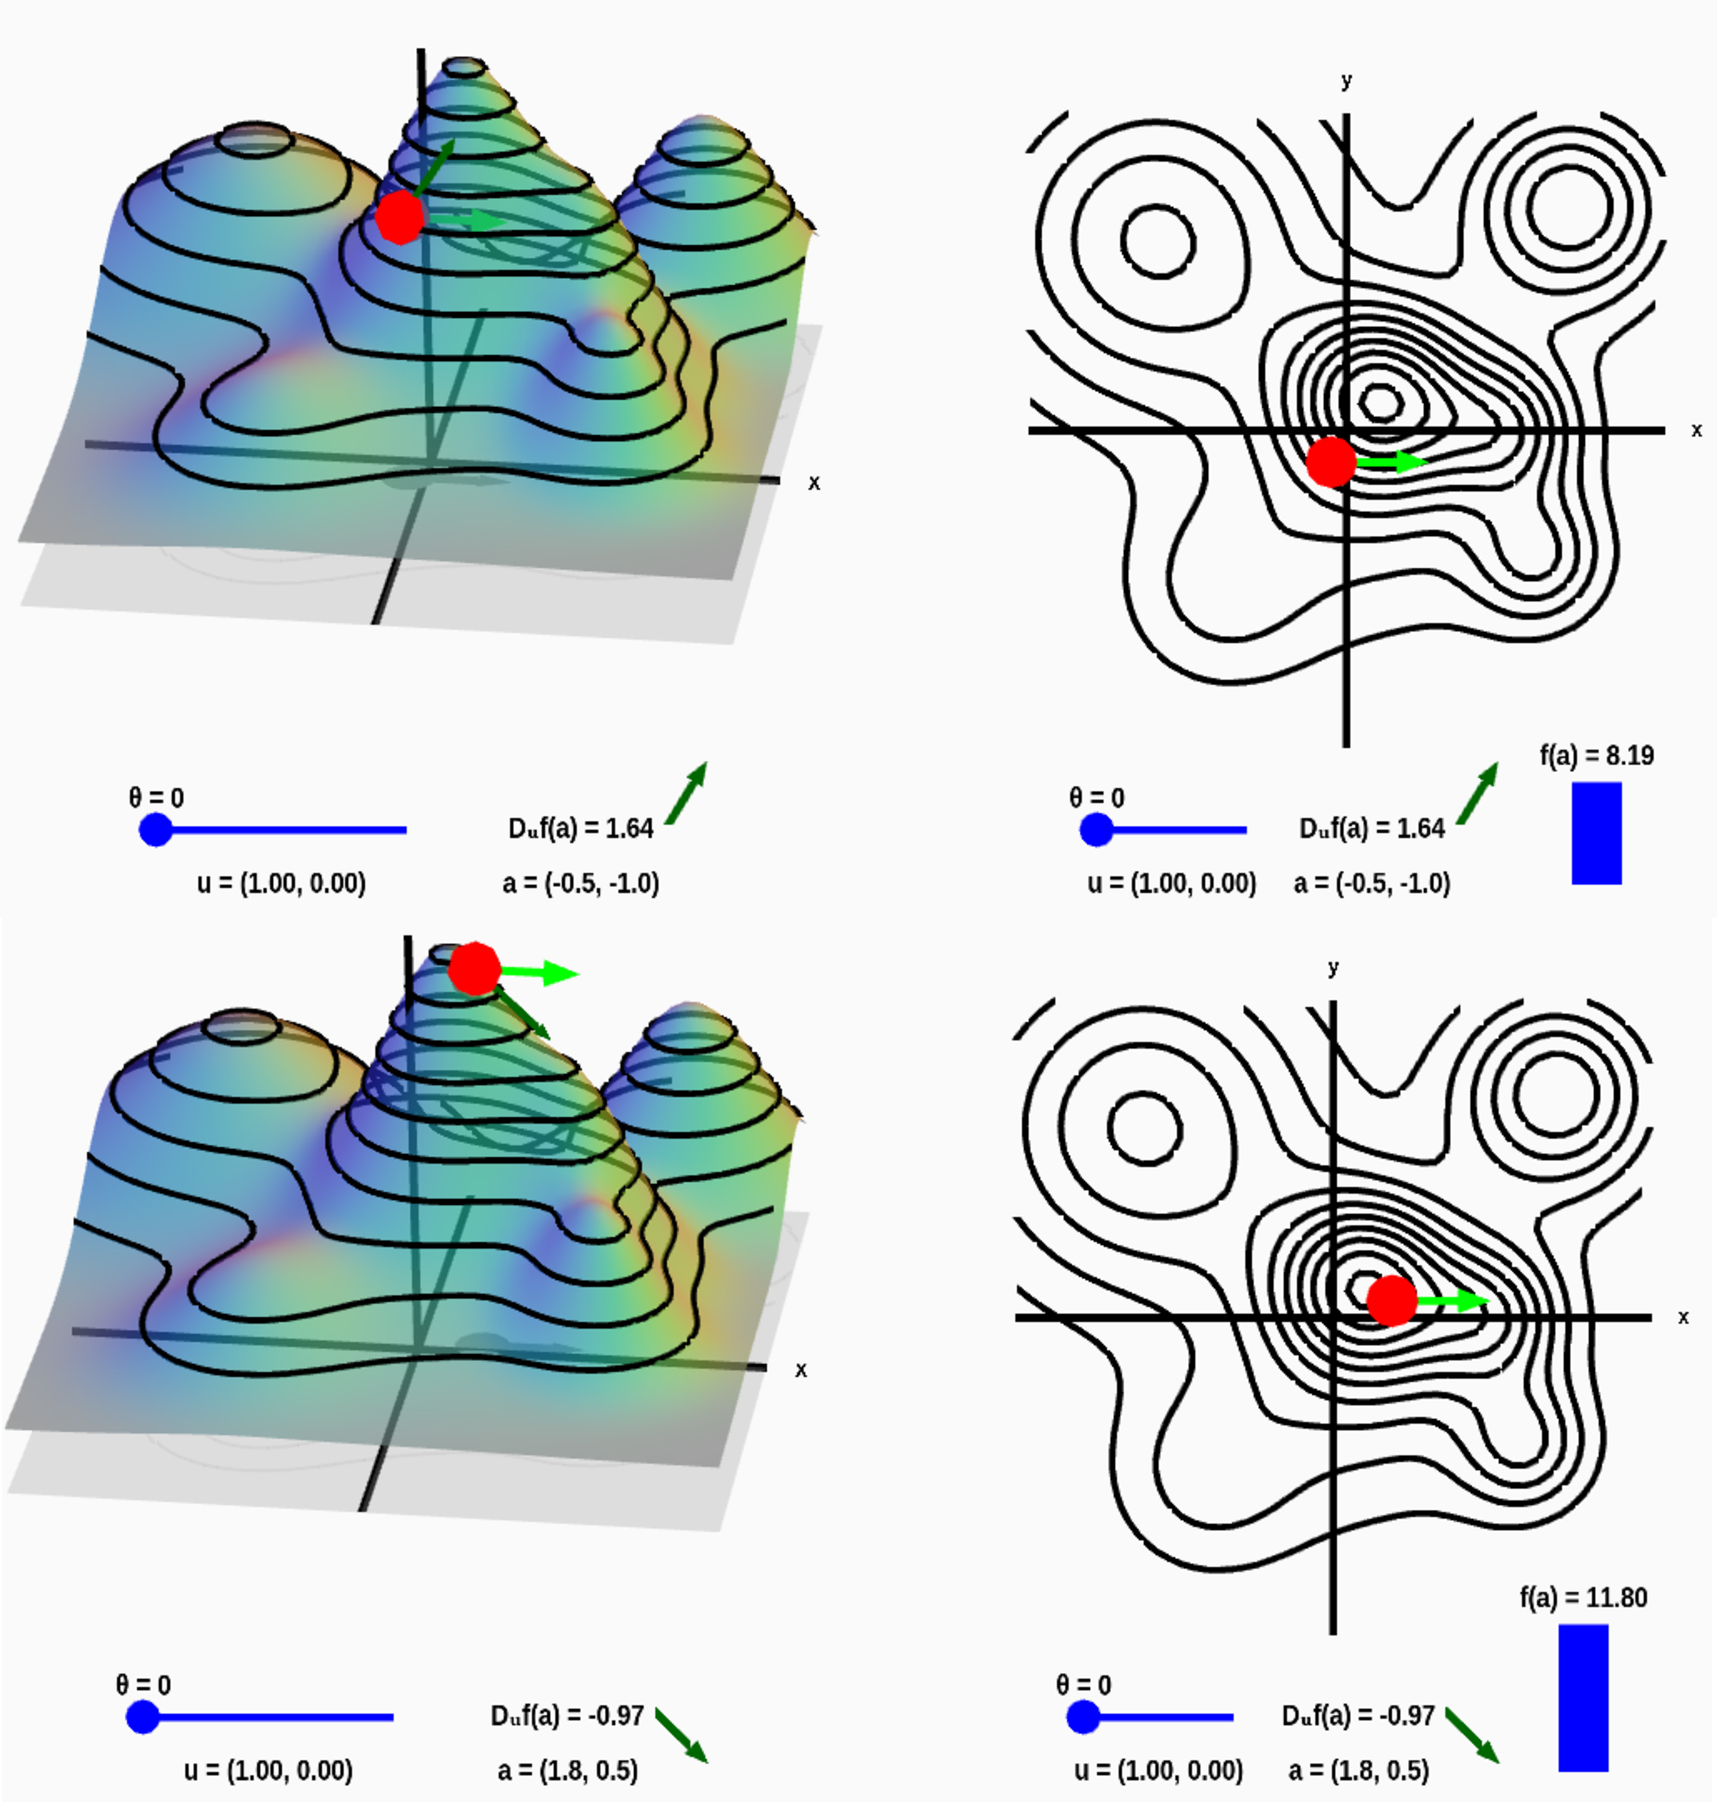
\includegraphics[scale=0.5]{directional-derivative-1.pdf}
\caption{\label{fig:directional_derivative_1}Directional derivative on a mountain\cite{mathInsight:DirectionalDerivative}. The height of a mountain range described by a function $f(x,y)$ is shown as surface plot in 3D (left), and a 2-D level curve plot (contour) (right). In each panel, a red point is the viewer, or the point where the directional derivative is to be evaluated. The directional derivative is computed in the direction of the 2D vector $\vec u$. The direction is illustrated by the light green vectors as well shown in the lower left. The direction of $\vec u$ is determined by the angle $\theta$ it makes with straight east (positive $x$ direction). The 2D point $\vec a$ where the directional derivative is computed is illustrated by the shadow of the red point on the $xy$-plane below the surface plot and by the red point itself on the level curve plot. The value of the directional derivative $D_{\vec u}f(\vec a)$ is shown at the bottom of the panel, along with the value of $\vec a$ itself. The value of $D_{\vec u}f(\vec a)$ is thes lope of the dark green vector to its right. This dark green vector is also shown emanating from the red point on the surface plot, where it is tangent to the surface, indicating that this slope is indeed the slope of the surface in the direction given by $\vec u$. The height of the surface $f(\vec a)$ is illustrated by the blue bar in the lower right.}
\end{figure}

In most cases, there is always one direction $\vec u$ where the directional derivative $D_{\vec u}f(\vec a)$ is the largest. This is the ``uphill'' direction. Let's call it the direction $\vec m$, and the maximal directional derivative $D_{\vec m}f(\vec a)$ are captured by something called the gradient of $f$, and denoted by $\nabla f(a)$. The gradient is a vector that points in the direction of $\vec m$ and whose magnitude is $D_{\vec m}f(\vec a)$. In other word: $\dfrac{\nabla f(\vec a)}{||\nabla f(\vec a)||} = \vec m$ and $||\nabla f(\vec a)|| = D_{\vec m}f(\vec a)$

Consider $\theta$ is the angle between the gradient $\nabla f(\vec a)$ and the direction vector $\vec u$. When $\theta = 0$ (or $\theta = 2\pi$), then $\vec u$ points in the same direction as the gradient. Also, then the directional derivative $D_{\vec u}f(\vec a)$ and the maginitude of the gradient $||\nabla f(\vec a)||$ are identical, i.e., $D_{\vec u}f(\vec a) = ||\nabla f(\vec a)||$

But, when $\theta = \pi$, then $\vec u$ points in the opposite direction of the gradient, and $D_{\vec u}f(\vec a) = -||\nabla f(\vec a)||$

Thus, for a fixed $\vec a$, the maximal value of $D_{\vec u}f(\vec a)$ occurs when $\vec u$ and $\nabla f(a)$ point in the same direction (i.e., when $\theta = 0$ or $\theta = 2\pi$), and the minimum value occurs when $\vec u$ and $\nabla f(\vec a)$ point in opposite directions (i.e., when $\theta = \pi$). Hence, $D_{\vec u}f(\vec a)$ always lies between $-||\nabla f(\vec a)||$ and $||\nabla f(\vec a)||$.

It turns out that the relationship between the gradient and the directional derivative can be summarized by the equation:
\begin{eqnarray}
\nonumber D_{\vec u}f(\vec a) &=& \nabla f(\vec a) \cdot \vec u\\
\nonumber &=& ||\nabla f(\vec a)|||| \vec u|| \cos\theta\\
\nonumber &=& ||\nabla f(\vec a)|| \cos\theta\\
\end{eqnarray}
where $\theta$ is the angle between $\vec u$ and the gradient $\nabla f(\vec a)$, and $\vec u$ is the unit vector.

The gradient always points in the direction where the mountain rises most steeply.

In a summary, given a multivariate scalar-valued function $f:\mathbb{R}^n\rightarrow \mathbb{R}$,
\begin{itemize}
	\item The directional derivative $D_{\vec u}f$ is a generalization of the partial derivative to the slope of $f$ in a direction of an arbitrary unit vector $\vec u$.
	\item The gradient $\nabla f$ is a vector that points in the direction of the greatest upward slope whose length is the directional derivative in that direction,
	\item The directional derivative is the dot product between the gradient and the unit vector: $D_{\vec u}f = \nabla f \cdot \vec u$
\end{itemize}

It is simple to calculate an expression for the gradient of a function, if we can remember what it means for a function to be differentiable. What does it mean for a function $f(\vec x)$ to be differentiable at the point $\vec x = \vec a$? The function must be locally be essentially linear, i.e., there must be a linear approximation
\[ L(\vec x) = f(\vec a) + Df(\vec a)(\vec x - \vec a) \]
that is very close to $f(\vec x)$ for all $\vec x$ near $\vec a$. The definition of differentiability means that, for all directions emanating out of $\vec a$, $f(\vec x)$ and $L(\vec x)$ have the same slope. We can therefore calculate the directional derivatives of $f$ at $\vec x$ using $L$ rather than $f$.

Using the definition of directional derivative, we can calculate the directional derivative of $f$ at $\vec a$ in the direction of $\vec u$:
\begin{eqnarray}
\nonumber D_{\vec u}f(\vec a) &=& D_{\vec u}L(\vec a)\\
\nonumber &=& \lim_{h\rightarrow 0}\dfrac{L(\vec a + h\vec u)-L(\vec a)}{h}\\
\nonumber &=& \lim_{h\rightarrow 0}\dfrac{\cancel{f(\vec a)}+Df(\vec a)(\cancel{\vec a} + h\vec u - \cancel{\vec a})-\cancel{f(\vec a)} - Df(\vec a)(\vec a-\vec a)}{h}\\
\nonumber &=& \lim_{h\rightarrow 0}\dfrac{Df(\vec a)\cancel{h}\vec u}{\cancel{h}}\\
\nonumber &=& \lim_{h\rightarrow 0}Df(\vec a)\vec u\\
\nonumber &=& Df(\vec a)\vec u\qquad (\text{setting $h=0$})
\end{eqnarray}
Since $Df(\vec x)$ is a $1\times n$ row vector and $\vec u$ is an $n\times 1$ column vector, the result is a scalar. We could rewrite this product as a dot-product between two vectors, by reforming the $1\times n$ matrix of partial derivatives into a vector. We denote the vector by $\nabla f$ and we call it the gradient. We obtain that the directional derivative is 
\[ D_{\vec u}f(\vec a) = \nabla f(\vec a)\cdot \vec u \]

Now, let's do some practice examples:\cite{mathInsight:DirectionalDerivativeExamples}.

\textbf{Example 1}: Let $f(x,y) = x^2y$. (a) Find $\nabla f(3,2)$. (b) Find the derivative of $f$ in the direction of (1,2) at the point (3,2).

\textbf{Solution:} (a) The gradient is the vector of the partial derivatives. That is:
\begin{eqnarray}
\nonumber \nabla f(x,y) = \begin{pmatrix}
\frac{\partial f}{\partial x}\\
\frac{\partial f}{\partial y}
\end{pmatrix} = \begin{pmatrix}
2xy\\
x^2
\end{pmatrix}
\end{eqnarray}
So, 
\begin{eqnarray}
\nonumber \nabla f(3,2) = \begin{pmatrix}
2.3.2\\
3^2
\end{pmatrix} = \begin{pmatrix}
12\\
9
\end{pmatrix} = 12\hat{i} + 9\hat{j}
\end{eqnarray}
(b) We need to find out the directional derivative $D_{\vec u}f(\vec a)$, where the unit vector in the direction of (1,2) is $\vec u=\frac{(1,2)}{\sqrt{1^2+2^2}} = (\frac{1}{\sqrt{5}},\frac{2}{\sqrt{5}}) = \frac{1}{\sqrt{5}}\hat{i}+\frac{2}{\sqrt{5}}\hat{j}$ and  $\vec a = (3,2)$.

So, using the relationship among directional derivative and the gradient, we can obtain the result:
\begin{eqnarray}
\nonumber D_{\vec u}f(\vec a) &=& \nabla f(\vec a)\cdot \vec u\\
\nonumber &=& (12\hat{i}+9\hat{j})\cdot (\frac{1}{\sqrt{5}}\hat{i}+\frac{2}{\sqrt{5}}\hat{j})\\
\nonumber &=& \frac{12}{\sqrt{5}} + \frac{18}{\sqrt{5}} = \frac{30}{\sqrt{5}}
\nonumber 
\end{eqnarray}
\textbf{Example 2}: For the $f$ in example 1, find the directional derivative of $f$ at the point (3,2) in the direction (2,1).

\textbf{Solution}: So, here the unit vector $\vec u$ gets changed to $\frac{(2,1)}{\sqrt{2^1+1^2}} = (\frac{2}{\sqrt{5}},\frac{1}{\sqrt{5}}) = \frac{2}{\sqrt{5}}\hat{i} + \frac{1}{\sqrt{5}}\hat{j}$, and the point $\vec a = (3,2)$ same as in example 1. We already calculated the gradient at that point which is $\nabla f(3,2) = 12\hat{i}+9\hat{j}$

So, we can compute the directional derivative by
\begin{eqnarray}
\nonumber D_{\vec u}f(\vec a) &=& \nabla f(\vec a)\cdot \vec u\\
\nonumber &=& (12\hat{i}+9\hat{j})\cdot (\frac{2}{\sqrt{5}}\hat{i} + \frac{1}{\sqrt{5}}\hat{j})\\
\nonumber &=& \frac{24}{\sqrt{5}} + \frac{9}{\sqrt{5}} = \frac{33}{\sqrt{5}}
\end{eqnarray}

\textbf{Example 3}: For the $f$ in example 1 at the point (3,2), (a) in which direction is the directional derivative maximal? (b) what is the value of the directional derivative in that direction, i.e., what is the maximal directional derivative of $f$ at point (3,2)?

\textbf{Solution}: (a) We know the gradient points are always in the direction of the maximal directional derivative. So since the gradient of $f$ at point (3,2) is $\nabla f(3,2) = 12\hat{i} + 9\hat{j} = (12,9)$, we will have the maximal directional derivative in this direction. So the answer is the unit vector in that direction, i.e., $\vec u = \frac{(12,9)}{\sqrt{12^2+9^2}} = (\frac{12}{15},\frac{9}{15}) = (\frac{4}{5},\frac{3}{5}) = \frac{4}{5}\hat{i}+\frac{3}{5}\hat{j}$

(b) The maximal directional derivative in the direction of $\vec u$ at point $\vec a =(3,2)$ would be
\begin{eqnarray}
\nonumber D_{\vec u}f(\vec a) &=& \nabla f(\vec a)\cdot \vec u\\
\nonumber &=& (12\hat{i}+9\hat{j})\cdot (\frac{4}{5}\hat{i} + \frac{3}{5}\hat{j})\\
\nonumber &=& \frac{48}{5} + \frac{27}{5} = \frac{75}{5} = 15 = ||\nabla f(3,2)|| = ||12\hat{i}+9\hat{j}|| =  \sqrt{12^2+9^2} = 15
\end{eqnarray}

\section{Gradient as a derivative}
A Gradient is the derivative of a scalar with respect to a vector. For vector $\vec x = (x_1, x_2, \cdots, x_n)^T$.
\begin{eqnarray}
\nonumber \dfrac{\partial f(\vec x)}{\partial \vec x} = \begin{pmatrix} \left[ \dfrac{\partial f(\vec x)}{\partial x_1}\right]\\
\left[ \dfrac{\partial f(\vec x)}{\partial x_2}\right]\\
\vdots\\
\left[ \dfrac{\partial f(\vec x)}{\partial x_n}\right] \end{pmatrix}
\end{eqnarray}
For Example, if we have a function: $f(\vec x) = x_1x^2_3 + x_1x^2_2 + x_2x^2_3 + x^2_1 + x^2_2 + x^2_3 + 2x_1x_2 + 2x_1x_3 + 2x_2x_3$, with $\vec x = (x_1, x_2, x_3)^T$.  Then the Gradient is:
\begin{eqnarray}
\nonumber \dfrac{\partial f(\vec x)}{\partial \vec x} &=& \begin{pmatrix}\left[ \dfrac{\partial f(\vec x)}{\partial x_1}\right]\\
\left[ \dfrac{\partial f(\vec x)}{\partial x_2}\right]\\
\left[ \dfrac{\partial f(\vec x)}{\partial x_3}\right]\end{pmatrix}\\
\nonumber &=& \begin{pmatrix}
x^2_3+x^2_2+2x_1+2x_2+2x_3\\
2x_1x_2+x^2_3+2x_2+2x_1+2x_3\\
2x_1x_3+2x_2x_3+2x_3+2x_1+2x_2
\end{pmatrix}
\end{eqnarray}

\section{Jacobian as a derivative}
A Jacobian is a derivative of a vector with respect to a transposed vector. For a vector $\vec x = (x_1, x_2, \cdots, x_n)^T$, and a $k$ dimensional function $\vec f = (f_1, f_2, \cdots, f_k)^T$, we have
\begin{eqnarray}
\nonumber \dfrac{\partial \overrightarrow{f(\vec{x})}}{\partial \vec x^T} = \begin{pmatrix}
\left[ \dfrac{\partial f_1(\vec x)}{\partial x_1}\right] & \left[ \dfrac{\partial f_1(\vec x)}{\partial x_2}\right] & \cdots & \left[ \dfrac{\partial f_1(\vec x)}{\partial x_n}\right]\\
\vdots & \vdots & \ddots & \vdots \\
\left[ \dfrac{\partial f_k(\vec x)}{\partial x_1}\right] & \left[ \dfrac{\partial f_k(\vec x)}{\partial x_2}\right] & \cdots & \left[ \dfrac{\partial f_k(\vec x)}{\partial x_n}\right]
\end{pmatrix}
\end{eqnarray}
For instance, if we have a function 
\[ 
\overrightarrow{f(\vec x)} = \begin{pmatrix}
3x^2_1 + x_2\\
ln(x_1) + x_3\\
sin(x_2) + cos(x_4)
\end{pmatrix}, \qquad \vec x= \begin{pmatrix}
x_1\\x_2\\x_3\\x_4
\end{pmatrix}
\]
Then the Jacobian is
\begin{eqnarray}
\nonumber \dfrac{\partial \overrightarrow{f(\vec{x})}}{\partial \vec x^T} = \begin{pmatrix}
\left[ \dfrac{\partial f_1(\vec x)}{\partial x_1}\right] & \left[ \dfrac{\partial f_1(\vec x)}{\partial x_2}\right] & \left[ \dfrac{\partial f_1(\vec x)}{\partial x_3}\right] & \left[ \dfrac{\partial f_1(\vec x)}{\partial x_4}\right]\\
\left[ \dfrac{\partial f_2(\vec x)}{\partial x_1}\right] & \left[ \dfrac{\partial f_2(\vec x)}{\partial x_2}\right] & \left[ \dfrac{\partial f_2(\vec x)}{\partial x_3}\right] & \left[ \dfrac{\partial f_2(\vec x)}{\partial x_4}\right]\\
\left[ \dfrac{\partial f_3(\vec x)}{\partial x_1}\right] & \left[ \dfrac{\partial f_3(\vec x)}{\partial x_2}\right] & \left[ \dfrac{\partial f_3(\vec x)}{\partial x_3}\right] & \left[ \dfrac{\partial f_3(\vec x)}{\partial x_4}\right] 
\end{pmatrix} = \begin{pmatrix}
6x_1 & 1 & 0 & 0\\
\frac{1}{x_1} & 0 & 1 & 0\\
0 & cos(x_2) & 0 & -sin(x_4)
\end{pmatrix}
\end{eqnarray}

\section{Hessian as a derivative}
The Hessian is the derivative of a Gradient with respect to a transposed vector. For a given vector $\vec x =(x_1, x_2, \cdots, x_n)^T$, we have the gradient
\begin{eqnarray}
\nonumber \dfrac{\partial f(\vec x)}{\partial \vec x} = \begin{pmatrix} \left[ \dfrac{\partial f(\vec x)}{\partial x_1}\right]\\
\left[ \dfrac{\partial f(\vec x)}{\partial x_2}\right]\\
\vdots\\
\left[ \dfrac{\partial f(\vec x)}{\partial x_n}\right] \end{pmatrix}
\end{eqnarray}
Then the Hessian would the derivative of this gradient with respect to $\vec x^T$.
\begin{eqnarray}
\nonumber \dfrac{\partial^2 f(\vec x)}{\partial \vec x\partial \vec x^T} = \begin{pmatrix} \left[ \dfrac{\partial f(\vec x)}{\partial x^2_1}\right] & \left[ \dfrac{\partial f(\vec x)}{\partial x_1 \partial x_2}\right] & \cdots & \left[ \dfrac{\partial f(\vec x)}{\partial x_1\partial x_n}\right]\\
\vdots & \vdots & \ddots & \vdots\\
\left[ \dfrac{\partial f(\vec x)}{\partial x_n\partial x_1}\right] & \left[ \dfrac{\partial f(\vec x)}{\partial x_n \partial x_2}\right] & \cdots & \left[ \dfrac{\partial f(\vec x)}{\partial x^2_n}\right]
 \end{pmatrix}
\end{eqnarray}
For instance, for function $f(\vec x) = x_1x^2_3 + x_1x^2_2 + x_2x^2_3 + x^2_1 + x^2_2 + x^2_3 + 2x_1x_2 + 2x_1x_3 + 2x_2x_3$, with $\vec x = (x_1, x_2, x_3)^T$, the Gradient we computed previously wass
\begin{eqnarray}
\nonumber \dfrac{\partial f(\vec x)}{\partial \vec x} &=& \begin{pmatrix}
x^2_3+x^2_2+2x_1+2x_2+2x_3\\
2x_1x_2+x^2_3+2x_2+2x_1+2x_3\\
2x_1x_3+2x_2x_3+2x_3+2x_1+2x_2
\end{pmatrix}
\end{eqnarray}
Hence, the Hessian would be
\begin{eqnarray}
\nonumber \dfrac{\partial^2 f(\vec x)}{\partial \vec x\partial \vec x^T} = \begin{pmatrix} \left[ \dfrac{\partial f(\vec x)}{\partial x^2_1}\right] & \left[ \dfrac{\partial f(\vec x)}{\partial x_1 \partial x_2}\right] & \left[ \dfrac{\partial f(\vec x)}{\partial x_1 \partial x_3}\right]\\
\left[ \dfrac{\partial f(\vec x)}{\partial x_2\partial x_1}\right] & \left[ \dfrac{\partial f(\vec x)}{\partial x^2_2}\right] & \left[ \dfrac{\partial f(\vec x)}{\partial x_2 \partial x_3}\right]\\
\left[ \dfrac{\partial f(\vec x)}{\partial x_3\partial x_1}\right] & \left[ \dfrac{\partial f(\vec x)}{\partial x_3 \partial x_2}\right] & \left[ \dfrac{\partial f(\vec x)}{\partial x^2_3}\right]
 \end{pmatrix} = \begin{pmatrix}2 & 2x_2+2 & 2x_3+2\\
 2x_2+2 & 2x_1+2 & 2x_3+2\\
 2x_3+2 & 2x_3+2 & 2x_1+2x_2+2
 \end{pmatrix}
\end{eqnarray}
%%%%%%%%%%%%%%%%%%%%%%%%%%%%%%%%%%%%%%%%%%%%%%%%%%%
	\bibliographystyle{IEEEtran}
	\bibliography{Report}

\end{document}
